%%%%%%%%%%%%%%%%%%%%%%%%%%%%%%%%%%%%%%%%%%%%%%%%%%%%%%%%%%%%%%%%%%%%%%%%
\NeedsTeXFormat{LaTeX2e}
\documentclass[11pt]{article}
\usepackage{amsmath,amssymb,amsthm}
\usepackage[margin=1.0in]{geometry}
\usepackage{amscd}
\usepackage{amsthm}
\usepackage{epsfig}
\allowdisplaybreaks
\setlength{\unitlength}{1mm}
%%%%%%%%%%%%%%%%%%%%%%%%%%%%%%%%%%%%%%%%%%%%%%%%%%%%%%%%%%%%%%%%%%%%%%%%
\makeindex
\begin{document}
\title{\bf {PURE DATA SPACES....DRAFT.}}
\author{%
  SAUL YOUSSEF%
  \hfil \\
  Department of Physics \\
  Boston University \\
}
\maketitle
\begin{abstract}
All about spaces.
\end{abstract}
%%%%%%%%%%%%%%%%%%%%%%%%%%%%%%%%%%%%%%%%%%%%%%%%%%%%%%%%%%%%%%%%%%%%%%%%

%%%%%%%%%%%%%%%%%%%%%%%%%%%%%%%%%%%%%%%%%%%%%%%%%%%%%%%%%%%%%%%%%%%%%%%%
\theoremstyle{definition}
\newtheorem{axiom}{Axiom}
\newtheorem*{axiom*}{Axiom}
\newtheorem*{fact}{Fact}
\newtheorem{theorem}{Theorem}[section]
\newtheorem{lemma}{Lemma}

\newtheorem{definition}{Definition}

\newtheorem*{remark}{}

\section{Overview}

....WRITE INTRODUCTION...

\begin{itemize}
\item Conceptual overview: small(est?) axiomatic system analogous to ZFC, where proof and computation are the same thing.
\item Point of the paper is to investigate the concept of a "Space" introduced in ref. 1.  This is analogous to ``Set'' or ``Category.''
\item Theme is to ``grow the simplest spaces organically'' and compare the simplest results with classical mathematics. 
\item Minimal container...associative data...semiring...analogous to sets or categories.
\end{itemize}

\section{Foundation}  

In \cite{PDF}, we argue that Mathematics and Computing as a whole can be captured within a small axiomatic framework, 
based on {\bf finite sequence} as the foundational concept.  Assuming that finite sequences are understood, {\it data} and {\it coda} are defined by 

\begin{definition} {{\bf Data} is a finite sequence of {\bf codas}, where each {\bf coda} is a pair of {\bf data}.}
\end{definition}

\noindent The two foundational operations defined on data are 1) concatenation of data $A$ and data $B$, written `$A\ B$', and 2) pairing of data $A$ and data $B$ as a coda, written with a colon `$A:B$'.   
By Definition 1, the empty sequence, written `()', qualifies as data and, therefore, () paired with itself is a coda, written `(():())' or `(:)'.  
Any finite sequence of codas is data, so, for example, (:)\ (:(:))\ ((:):(:(:))) is  
data consisting of a sequence of three codas.  We can think of this as {\it pure data} since it is ``data made of nothing.''  
By convention, the colon binds from the right first and binds less strongly than concatenation, so that $A:B:C$ is defined to be $(A:(B:C))$ and $A:B\ C$ is defined to be $(A:(B\ C))$.  
Data is typically written with upper case, and codas are typically written in lower case.  
To indicate the left and right data of a coda, we sometimes use L/R superscripts so, for any coda $c$, $c=(c^L:c^R)$. 

     All meaning within the system is determined by a chosen partial function from coda to data called a {\it context}. 
Contexts are partially ordered by inclusion, so if $\delta$ and $\delta'$ are contexts, $\delta\le\delta'$ if $\delta$ and $\delta'$ are equal on the domain of $\delta$.  
Given a context $\delta$, equality of data is the equivalence generated by $c\sim \delta(c)$ for any coda $c$, and by compatibility with concatenation and colon in the sense that 
if $A\sim B$, then $(A\ X)\sim (B\ X)$, $(X\ A)\sim (X\ B)$, $(A:X)\sim (B:X)$ and $(X:A)\sim(X:B)$ for any data $X$.  This relation $A\sim B$ is denoted $A{\overset\delta =}B$, 
or simply $A=B$ when the context is unambiguous.   
It follows that if $\delta\leq\delta'$, then $A{\overset\delta =}B$ implies $A{\overset{\delta'} =}B$.  We say that if $A$ and $B$ are equal then they are ``always equal,'' thinking 
of moving from $\delta$ to $\delta'$ as the passage of ``time."  The fixed points of a context $\delta$ are {\it atoms}.  Note that if $c$ is an atom in context $\delta$, 
and if $\delta\leq\delta'$, then $c$ is still an atom a context in $\delta'$.  Thus, atoms are ``permanent" and if $c$ is an atom, $c$ is ``always" an atom.  

\begin{definition}
{Within a given context $\delta$, coda $c$ is an {\bf atom} if $\delta:c\mapsto c$.  If data $A$ contains an atom in its sequence, $A$ is {\bf atomic} data. 
Data $A$ is {\bf invariant} if every coda $a$ in the sequence of $A$ is an atom and if $a^L$ and $a^R$ are both {\bf invariant}. }
\end{definition}
\noindent It follows from the definition that empty data is invariant and atoms $a$ and $b$ are equal if and only if $a^L=b^L$ and $a^R=b^R$.  If $a$ and $b$ are atoms, 
$A$ and $B$ are data, then $(a\ A)=(b\ B)$ and $(A\ a)=(B\ b)$, if and only if $a=b$ and $A=B$.  If $A=B$ and $A$ and $B$ are invariant, then $A$ and 
$B$ are identical as pure data [proof].

\section{Genesis}

    In the proposed framework, all mathematical objects are pure data and all meaning is defined by a chosen context $\delta$ and its corresponding equivalence.  
A {\bf proof} in $\delta$, for example, is just a sequence $A_1{\overset \delta =}$ $A_2 {\overset \delta =} \dots {\overset \delta =}$$A_n$ which can be viewed either as proving $A_n$ 
given $A_1$ or as a computation $A_1\mapsto A_n$. 
The immediate issue is how to choose $\delta$.  
    
     In the beginning, there are no definitions, and the corresponding context is the empty partial function $\delta_0$.  
Since the domain of $\delta_0$ is empty, it has no fixed points and, therefore no atoms.  Thus, the empty sequence is the only invariant, 
$X{\overset \delta =}X$ is the only valid proof, and the only valid 
 computations do nothing $X\mapsto X$ for any data $X$.
To define a non-empty context $\delta_0\le\delta$, we need, at least, an invariant specification of the domain of $\delta$ as a partial function.    
Since the empty sequence is the only invariant, the only way to specify if a coda (A:B) is to be in the domain of $\delta$ is 
to require either A or B or both to be the empty sequence. In each of these cases, the coda (:) is within the domain of $\delta$, and so we must, in any case, 
decide on what (:) maps to.  There are three possibilities; 
\begin{itemize}
\item[] choice 1: {$\delta: (:) \mapsto ()$},
\item[] choice 2: {$\delta: (:) \mapsto (:)$}, or 
\item[] choice 3: {$\delta: (:) \mapsto \ anything\ other\ than\ ()\ or\ (:)$}. 
\end{itemize}
Since pure data is ``made of (:)'', choice 1 trivially causes all data to be equal to the empty sequence. 
On the other hand, choice 3 would mean that for any non-empty data $A$, the number of (:) atoms in $A$ grows without limit.  This would mean, for instance, 
that nocomputation could produce a final result.  Thus, we are constrained to choice 2, where (:) is an invariant atom in $\delta$, and, therefore an atom in 
any context $\delta\leq\delta'$ as well.  It is convenient to generalize choice 2 and to let $\delta$:(:$X$)$\mapsto$ (:$X$) for all data $X$, since this provides a 
supply of invariant atoms (:), (:(:)), (:(:) (:)),$\dots$ which can be used to expand the domain of $\delta$.  

We adopt a convention for expanding the domain of $\delta$ while preserving context partial ordering. 
A context of the form 
\begin{equation}
	\delta_a: (a\ A:B) \mapsto \delta_a(A,B)
\end{equation}
for some invariant atom $a$ is called a {\bf definition}.  We conventionally restrict ourselves to 
contexts $\delta\cup\delta_a\cup\delta_b\cup\dots$ where $a$ is an invariant atom in $\delta$, $b$ is an invariant atom in $\delta\cup\delta_a$, $c$ is an invariant atom in $\delta\cup\delta_a\cup\delta_b$ and so forth.  By requiring $a$, $b$,\dots to be disjoint, we maintain the context partial ordering.  

\section{Definitions}

     Before proceeding to mathematical exploration, we need to add enough expressive power to the original context $\delta$.  To do this, 
we introduce minimal definitions using the mechanism explained in the previous section.  

\begin{enumerate}
\item {Define ``bits'', ``bytes'' and ``byte sequences'' so that words are single atoms, so that $a$ can be a word in future definitions $\delta_a$.}
\item {Define all of the naturally occurring combinatoric operations given two finite sequences $A$ and $B$.  For example $\delta_{\rm ap}$
maps (ap $A$ : b$_1$\ b$_2$ $\dots$ b$_n$) to ($A$:b$_1$)\ ($A$:b$_2$)$\dots$ ($A$:b$_n$), so that ap ``applies $A$ to each atom of input.'' }
\item {Define a minimal internal language $\delta_{\{\}}$ so that a coda $(\{\texttt{language expression}\}\ A : B)$ is mapped to data as described by 
the expression and possibly using data $A$ and data $B$.}
\item {Include definitions giving direct access to context-level values.  This include a Boolean definition $\delta_{\rm bool}$ to determine if data is empty, 
$\delta_{=}$ to test if two data are equal in $\delta$, and $\delta_{\rm def}$ to add definitions via Equation 1.} 
\end{enumerate}
These are meant to be a minimal collection of definitions, including only the minimal inevitable finite sequence concepts and, more generally, 
the combinatorics of Equation X.  There are intentionally no definitions which presume underlying arithmetical operations.  A natural number, 
`123`, for instance is a single atom byte sequence and there is no definition which implies interpreting this as a number in the usual way.  The idea is
to allow natural numbers and whatever else to emerge ``organically.'' 
There are approximately fifty definitions needed to create a basic system system.  We define some here for orientation.  More details can be found in the Glossary.  

\subsection{Bits, Bytes and Byte sequences}

If `a' is an invariant atom, a new atom with domain (a A:B) is defined by $\delta_a: (a\ A:B)\mapsto (a\ A:B)$, so that $\delta_a$ is a fixed point on its domain.  
We may refer to these as ``a-atoms."  For readability convenience, we define (:)-atoms, ((:):)-atoms and ((:):(:))-atoms to hold bits, bytes and words respectively
so that text strings are invariant atoms within the context $\delta\cup\delta_{(:)}\cup\delta_{((:):)}\cup\delta_{((:):(:))}$.

\subsection{Combinatorics} 

Given that text strings are invariant atoms, we can add definitions with readable names.  Define the identity `pass' so that (${\rm pass}:X$=$X$) for all data $X$.  
\begin{itemize}
\item{$\delta_{\rm pass}$ : ({\rm pass} A:B) $\mapsto$ B}
\end{itemize}
and define `null' so that (${\rm null}:X$=$()$) for all $X$.
\begin{itemize}
\item{$\delta_{\rm null}$ : ({\rm null} A:B) $\mapsto$ ()}
\end{itemize}
It is convenient to define ``getting the A and B components of a coda'' like so
\begin{itemize}
\item{$\delta_{\rm left}$ : ({\rm left} A:B) $\mapsto$ A} 
\item{$\delta_{\rm right}$ : ({\rm right} A:B) $\mapsto$ B} 
\end{itemize}
We proceed to define the minimal combinatorics involving of A and B as finite sequences.  These don't have 
commonly understood names, so we are forced to invent new names.  For example the name `ap' is meant to suggest the 
concept ``apply A to each atom of B" is expressed by the definition.  
\begin{itemize}
\item{$\delta_{\rm ap}$ : ({\rm ap} A : b B) $\mapsto$ (A:b) ({\rm ap} A : B)}
\item{$\delta_{\rm ap}$ : ({\rm ap} A : ()) $\mapsto$ ()} 
\end{itemize} 
The domain of $\delta_{\rm ap}$ is defined with the assumption that $b$ is an atom, so the domain of the first branch of $\delta_{\rm ap}$ is exactly 
codas $({\rm ap}\ A,B)$ where $B$ starts with an atom.  By definition, if we list multiple ``branches'' as in this case, the first branch in the domain applies.  

\subsection{Language} 

Axiomatic systems like ZFC[ref] or dependent type theories[ref] are formal languages.  There is an alphabet, special symbols, and syntax rules 
for defining valid expressions.  Our approach avoids this by defining a language as just one more definition like any other.  The basic idea is to 
define minimalist language, mainly giving access to the two foundational operations via text blank space (for concatentation) and text colon (for pairing to data as a coda).  So, the idea is 
\begin{itemize}
\item {$\delta_{\{\}}$ : (\{x\ y\} A : B) $\mapsto$ (\{x\} A:B) (\{y\} A:B)}
\item {$\delta_{\{\}}$ : (\{x:y\} A : B) $\mapsto$ (\{x\} A:B) : (\{y\} A:B)}
\end{itemize}
where x and y are byte sequences as defined above.  As written, this is ambiguous since $x$ and $y$ may contain space and colon characters, but 
these ambiguities can be resolved just by choosing and order, thus forcing the language into one definition 
$\delta_{\{\}}$.  This definition includes 
\begin{itemize}
\item {$\delta_{\{\}}$ : (\{A\} A : B) $\mapsto$ A}
\item {$\delta_{\{\}}$ : (\{B\} A : B) $\mapsto$ B}
\end{itemize}
so that A and B have special meaning in the language.  As a result, for example, (\{B\}:1 2 3)=1 2 3, (\{B B\}:1 2 3)=1 2 3 1 2 3, and (\{A B\} a b : 1 2)=a b 1 2.  

     Given a language expression in the form of byte sequence data $L$, the corresponding data is, simply, ($L$:).  Every sequence of bytes is a valid language 
expression, so there is actually no need to define or check for syntax errors.  Similarly, an {\it evaluation} of ($L$:) is merely some sequence 
($L$:)=$D_1$=$D_2$=$\dots$=$D_n$ producing an ``answer'' $D_n$.  Typically, this is done with a simple strategy based on applying $\delta$ whenever 
possible or up to time or space limits.  This also means that there is also no such thing as a ``run time error.''    

\subsection{System} 

    The most basic question to ask about data is whether it is empty or not.  This is captured by the definition $\delta_{\rm bool}$, defined 
so that (bool:B) is () if B is empty (``true'') and (bool:B)=(:) if B is atomic (``false'').
\begin{itemize}
\item {$\delta_{\rm bool}$ : ({\rm bool} A : B) $\mapsto$ () if $B$ is empty, (:) if $B$ is atomic.}
\item {$\delta_{\rm not}$ : ({\rm not} A : B) $\mapsto$ (:) if $B$ is empty, () if $B$ is atomic.} 
\end{itemize} 
The equality defined by the context $\delta$ is available within $\delta$ via the following definition:
\begin{itemize}
\item {$\delta_{=}$ : (= A : ()) $\mapsto$ A}
\item {$\delta_{=}$ : (= (): A) $\mapsto$ A}
\end{itemize}
and if a and b are atoms, 
\begin{itemize}
\item {$\delta_{=}$ : (= a A : b B) $\mapsto$ (= a:b) (=A:B)}
\item {$\delta_{=}$ : (= A a : B b) $\mapsto$ (=A:B) (= a:b)}
\end{itemize}
so, if $(A:B)$ is empty, $A$ and $B$ are ``always'' equal and if $(A:B)$ is atomic, $A$ and $B$ are ``never'' equal.  The full language has a little bit 
of syntactic sugar, so one can write (A=B) instead of (= A:B) [ref]. 

New definitions can also be added to context via  
\begin{itemize}
\item {$\delta_{def}$ : ({\rm def} \texttt{name} A : B} $\mapsto$ ())
\end{itemize}
which is defined to be in domain as a partial function if \texttt{name} is not already in the current context, and, in that case, it adds the following definition
to context.
\begin{itemize}
\item {$\delta_{\texttt{name}}$:(\texttt{name}\ $A'$:$B'$) $\mapsto$ ($B\ A'$:$B'$)}
\end{itemize}
so, for instance (def first2 : {first 2 : B}), means that (first2 : a b c d) is interpreted as (\{first 2:B\} : a b c d) which is equal to the data (a b).   

We take this as the ``organic'' base of naturally occurring 
definitions plus the language will be a starting point in searching for the ``spaces'' defined in section 5.  Further definitions used in the text can be found in 
the Glossary.  Examples, tutorials, a complete definition of the language, and software can be 
found in reference [x]. 

\section{Global Structure} 

    Pure data has a global structure in the sense that the foundational operations $(A\ B)$ and $(A:B)$ are defined for any data $A$, $B$.  
This suggests defining a corresponding associative product $(A\cdot B)$ and associative sum $(A+B)$ by    
\begin{equation}
(A \cdot B):X = A:B:X 
\end{equation}
\begin{equation}
(A+B):X = (A:X)\ (B:X) 
\end{equation}
for all data $X$. This product distributes over the sum, from the right only, so we have 
\begin{equation}
(A+B)\cdot C=(A\cdot C)+(B\cdot C) 
\end{equation}
for any data $A$, $B$, and $C$.
Since $({\rm pass}\cdot A)$=$(A\cdot {\rm pass})$=$A$ and $(A+{\rm null})$=$({\rm null}+A)$=$A$ for any $A$, (pass) and (null) are the units of data composition and 
data addition respectively.  
Following standard terminology, we say that $A$ is {\it idempotent} if $A\cdot A$=$A$, is an {\it involution} if $A\cdot A$=$1$, and $A$ has an {\it inverse} if $A\cdot A'$=$A'\cdot A$=$1$ for some data $A'$.   
In the case of a {\it product}  A=$A_n\cdot\dots\cdot A_1$, we say that A {\it starts with} $A_1$ and {\it ends with} $A_n$.   

Data $A$ is called {\it algebraic} or {\it commutative} if $A:X\ Y$=$A:Y\ X$ for all $X$, $Y$.  Data $A$ is 
{\it distributive} if $A:X\ Y$=$(A:X)\ (A:Y)$ for all $X$ and for all $Y$.  
Data $A$ defines a binary operator on data via ($X{\overset A\ast}Y)=(A:X\ Y)$.  Since ${\overset A\ast}$ is associative if and only if 
 ($A$:$X$\ $Y$)=($A$:($A$:$X$)\ $Y$)=($A$:$X$ ($A$:$Y$)) for all $X$,$Y$ we say that data $A$ is {\it associative} if it has this property.  
 
Algebraic and distributive data foreshadow a theme where these two properties make data mathematically interesting for complementary reasons.  
Algebraic data has, in a sense, ``transcended finite sequence," the foundational concept of the system and has a platonic existence in 
that sense.  Distributive data, on the other hand, is maximally sequence dependent, but it may also be mathematically interesting since 
such data is a ``morphism of finite sequence.''   
 
\section{Spaces}

      A basic requirement for useful mathematics is to have a way to define and refer to collections.  
Within the framework of pure data, however, there is only one ``substance'' to work with.  All mathematical objects are merely data and 
all collections of mathematical objects are also merely data.  
Thus, we are lead to ask, given some data $S$, how could $S$ represent a collection of other data?  
There are a couple of plausible ways to do this.  
\begin{itemize} 
\item The collection corresponding to $S$ would be the collection of data ($S$:$X$) for any data $X$;
\item The collection corresponding to $S$ would be the collection of all of the fixed points of $S$.  
\end{itemize}
These ideas coincide if we require $S$ to be idempotent, so that ($S$:$X$) is automatically a fixed point.  It is natural to also expect compatibility with 
sequences in the sense that if ($S$:$X$) is in the collection and ($S$:$Y$) is in the collection, then ($S$:$X$) ($S$:$Y$) is also in the collection.  
This is guaranteed if we require 
\begin{equation}
(S : X\ Y) = S : (S:X)\ (S:Y)
\end{equation}
for all data $X$, $Y$.  
Note that data $S$ is idempotent and satisfies Equation 4 if and only if $S$ is associative, and so we are lead 
to a simple definition.
\begin{definition} Data $S$ is a {\bf space} if $S$ is associative.
\end{definition}
\noindent If $S$ is a space, we say that any data ($S$:$X$) is {\it in} $S$.  
The data ($S$:) is called the {\it neutral data} of $S$.  

Examples of spaces can be found in the basic definitions, including `pass`, `null` and `bool`.  More examples come from 
noting that any data which is both idempotent and distributive is a space.  Thus, if $J$ is idempotent, then (ap\ $J$) is idempotent and 
distributive, and is, therefore, a space.  If spaces $S$ and $T$ commute, then $S\cdot T$ is a space.    

\subsection{Morphisms} 

A product $F$ that starts with space $S$ and ends with space $T$ is a {\it morphism} from $S$ to $T$ and can be written $S{\overset F\longrightarrow}T$.
Since spaces are idempotent, $F$=($F\cdot S$)=($T\cdot F$).  Since $T\cdot S$ is a morphism from $S$ to $T$, morphisms always exist.  
Since the product is associative, morphisms can be composed, so that if $S{\overset F\longrightarrow}T$ and 
$T{\overset G\longrightarrow}U$, then $S{\overset {G\cdot F}\longrightarrow}U$.  
If $F$ and $G$ are morphisms from $S$ to $T$, we can also define a {\it sum of morphisms} by $F \oplus G = T\cdot (F+G)$, so that 
$S{\overset {F\oplus G}\longrightarrow}T$.  A morphism from a space to itself is called an {\it endomorphism}. 

    Since $T\cdot X\cdot S$ is a morphism from $S$ to $T$ for any data $X$, a morphism can define any function.  Special morphisms which 
``preserve the structure'' of $S$ and $T$ can be defined as follows.  A morphism $S{\overset H\longrightarrow}T$ is a {\it homomorphism} if 
\begin{equation}
H\cdot (f\oplus_S g) = (H\cdot f) \oplus_T (H\cdot g) 
\end{equation}
for all endomorphisms $f$ and $g$ of $S$.  Compare with morphisms that happen to also be a space.  Morphism $S{\overset U\longrightarrow}T$ is a space if and only if 
\begin{equation}
U\cdot (f\oplus_S g) = U\cdot ((U\cdot f) \oplus_T (U\cdot g)) 
\end{equation}
for all endomorphisms $f$ and $g$ of $S$.  Thus, any idempotent homomorphism is a space.  
Note that homomorphisms are closed under composition, but the composition of two spaces is a space 
only if the two spaces commute.  

\subsection{Spaces are Semirings} 

     Consider the endomorphisms of a fixed space $S$.  Since $S$ itself is a product starting at $S$ and ending at $S$, $S$ qualifies as an endomorphism of itself.  	
 Since ($S\cdot f$)=($f\cdot S$)=$f$ for any endomorphism $f$, $S$ is ``its own identity morphism.''  The endomorphisms 
of $S$ are closed under both composition and addition, with addition defined by $f\oplus g$ = $S\cdot(f+g)\cdot S$ = $S\cdot(f+g)$.  
Thus, the endomorphisms of $S$ are a `semiring' with composition and addition and with $1$=($S\cdot {\rm pass}\cdot S$)=$S$ and with 
$0$=($S\cdot {\rm null}\cdot S$)=($S\cdot {\rm null}$).  

\begin{definition}
A {\bf semiring} is a set with associative addition and multiplication (denoted $f\oplus g$ and $f\cdot g$), with additive and 
multiplicative identities {\bf 0} and {\bf 1} satisfying $f\oplus 0$=$f$=$0\oplus f$ and $f\cdot 1$=$f$=$1\cdot f$ for all $f$ in the semiring, and where 
$(f\oplus g)\cdot h$=$(f\cdot h)\oplus (g\cdot h)$ for all $f$, $g$, and $h$ in the semiring.  
A subset of a semiring $S$ which contains 0 and 1 and is closed under addition and multiplication is a {\bf subsemiring} of $S$.   
\end{definition} 
\noindent 
Note that the semiring of space $S$ has 1=0 if and only if $S$ is a constant space.  These spaces 
are (const $K$) for any chosen data $K$ including (const ())=null.
It is easy to verify that the semiring of the space (pass) is exactly the the global algebra defined in Section X.  Since isomorphic spaces have 
isomorphic semirings, understanding the semiring of a space is mainly what we aim for in the examples which follow.  Before going to examples, however, it is helpful 
to identify semiring features of interest. 

Consider the semiring of a fixed space $S$.  
\begin{itemize}

\item{{\bf Subspaces.} If an endomorphism $s$ of $S$ happens to also be a space, we say that $s$ is a {\it subspace} of $S$.  The name ``subspace'' is justified because every data contained in $s$ is also contained in $S$, and every endomorphism $s\cdot$X$\cdot s$ of $s$ is also an endomorphism of $S$.  
Subspaces partially distribute from the left as with $s\cdot(f\oplus g)$=$s\cdot((s\cdot f)\oplus(s\cdot g))$.
Every space has subspaces $1$ (the whole space), and $0$, the constant neutral space.  If subspace $s$ is not equal to $S$, $s$ is a {\it proper} subspace.} 

\item{{\bf Constants.}  An endomorphism $k$ of $S$ satisfying $k\cdot 0$=$k$ is a {\bf constant} subspace of $S$.  There is one such constant for each 
data in $S$.  Since $k\cdot f$ and $k\oplus l$ are constants for 
constant $k$ and $l$ and for any endomorphism $f$, the constants of $S$ are a left-ideal of the semiring of $S$.} 

\item{{\bf Homomorphisms.}  By Equation 5, the homomorphisms of $S$ are exactly the endomorphisms which distribute over addition from
both the left and from the right.  The endomorphisms 0 and 1 are homomorphisms.  If $f$ and $g$ are homomorphisms of $S$, then 
$f\cdot g$ is a homomorphism.  If $S$ is algebraic, the homomorphisms are a subsemiring of the semiring of $S$.} 

\item {{\bf Group of units}. The collection of endomorphisms with multiplicative inverses is called the {\it group of units} of the space $S$.} 

\item{{\bf Central endomorphisms}.  Endomorphisms which commute with the group of units are {\it central endomorphisms}.  The endomorphisms 0 and 1 
are central.  If $f$ and $g$ are central endomorphisms, then $f\cdot g$ is a central endomorphism.  If $f$ and $g$ are {\it central homomorphisms}, then 
$f\oplus g$ is also a central homomorphism.  Thus, the central homomorphisms of $S$ are a subsemiring of the semiring of $S$.}

\item{{\bf Neutral spaces and sets}. If addition in $S$ allows left and right cancellation ($f\oplus g=f\oplus h$ implies $g=h$ and $g\oplus f=h\oplus f$ implies $g=h$), 
$S$ is a {\it neutral} space.  The neutrality of $S$ guarantees $h\cdot 0$=0 for homomorphism $h$, and guarantees that if $f\oplus f$=$f$, then $f=0$. 
At the other extreme, if $f\oplus f$=$f$ is true for all endomorphisms and if $S$ is algebraic, then $S$ is a {\it set}.} 

\item{{\bf Positive spaces}.  If endomorphisms cannot cancel in the sense that $f\oplus g$=0 implies $f$=$g$=0, $S$ is a {\it positive} space.  If  
non-zero endomorphisms $f$ and $g$ imply that $f\cdot g$ is also non-zero, then $S$ is a {\it non-zero preserving} space.} 

\item{{\bf Idempotents}.  Define a relation ${\overset i \leq}$ on the endomorphisms of $S$ by $f{\overset i \leq}g$ if ($f\cdot g$)=$f$.  The equivalence 
classes of the corresponding symmetric relation $f{\overset i \sim} g$ contain all the idempotent endomorphisms, since $f{\overset i\sim}g$ implies that 
both $f$ and $g$ are idempotent.  In this {\it idempotent order}, 1 is the maximum endomorphism and the constant endomorphisms are minimal.}

\end{itemize} 
In the case where $S$ is distributive, $(f\oplus g)$ = $(f+g)$ for $f$, $g$ endomorphisms of $S$.  This means that the homomorphisms of $S$ are 
the distributive endomorphism.  If the group of units of $S$ includes permutations, then the central homomorphisms are algebraic.  This illustrates 
the generalization of the earlier remark about algebraic and distributive data being mathematically interesting for complementary reasons.  Central 
endomorphisms are the generalization of algebraic data and homomorphisms are the generalization of distributive data.  Naturally, one suspects 
that the central homomorphisms of a space will be particularly interesting. 

\subsection{Isomorphic Spaces have Isomorphic Semirings} 

The fact that homomorphisms compose suggests adapting definitions from Category Theory.  
We say, for instance, that spaces $S$ and $T$ are {\it isomorphic} if the diagram of Figure X commutes for homomorphisms 
$h$ and $h'$.  
\begin{figure}[h]
\centering
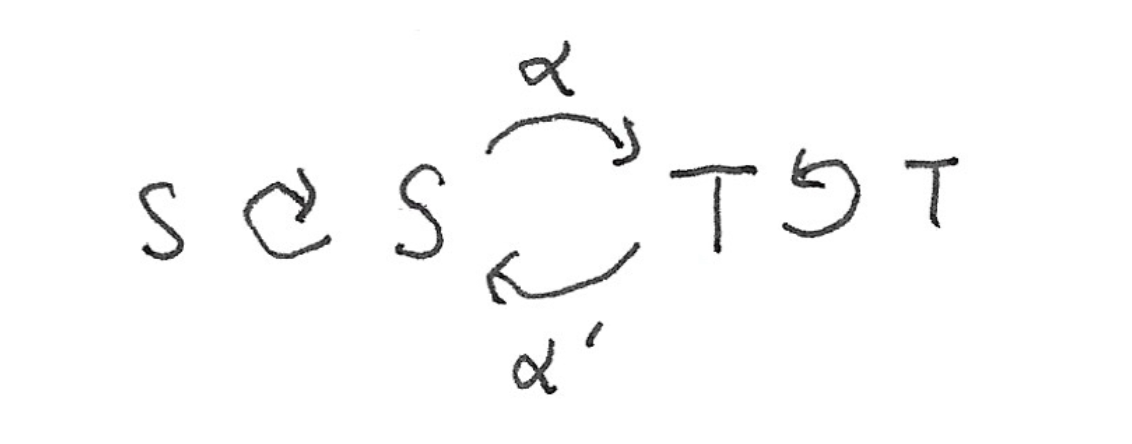
\includegraphics[width=0.4\textwidth]{isomorphism.png}
\caption{{\it In a definition adopted from Category Theory, spaces S and T are isomorphic if the diagram commutes for some homomorphisms $\alpha$ and $\alpha'$.}}
\end{figure}
where we have used $S$ and $T$ instead of respective ``identity morphisms."  Given an isomorphism as in Figure X, the bijection $f\mapsto h'\cdot f \cdot h$ is 
a semiring isomorphism, preserving product, sum, 1 and 0, so that isomorphic spaces have the same features defined in the previous section, since 
these are all defined with semiring operations.  A homomorphism $h$ where $h\cdot \alpha=h\cdot \beta$ implies $\alpha=\beta$ is a {\it monomorphism} and 
and if $\alpha\cdot h=\beta\cdot h$ implies $\alpha=\beta$, $h$ is an {\it epimorphism}.  

\subsection{Spaces can be Semialgebras} 

The semiring of a space $S$ is close to the structure of an ``algebra'' in standard mathematics.  There is a binary operation $f\oplus g$, so 
constants of the space can be added.  Homomorphisms have the property that they map constants to constants and are distributive with 
$h\cdot (k\oplus l)$ equal to $(h\cdot k)\oplus (h\cdot l)$ so homomorphisms of $S$ are like a module over the constants of $S$.  This would 
be an algebra in the ordinary sense except that homomorphisms might not be constants.  This suggests a definition 

\begin{definition}
A space $S$ is a {\bf semialgebra} if the homomorphisms of $S$ are bijectively equivalent to the constants of $S$.
A space $S$ is a {\bf central semialgebra} if the central homomorphisms of $S$ are bijectively equivalent to the constants of $S$.
\end{definition}
\noindent Since pure data is meant to include all mathematical objects, we might expect that important algebras of standard 
mathematics could appear semialgebras.  Whether this is true or not will be part of our investigation. 

\subsection{Subspaces are Substructures} 

Suppose that space $S$ has subspace $s$ and space $T$ has subspace $t$, and suppose that $F$=$t\cdot X\cdot s$ is a morphism from $s$ to $t$.   
Since ($t\cdot X\cdot s$) = ($T\cdot t \cdot X\cdot s\cdot S$), 
$F$ is also a morphism from $S$ to $T$, with the extra property that $F$ respects the structure of $s$ and $t$ in the sense that $t\cdot F=F\cdot s$.  
If a space has multiple subspaces, each commuting pair of subspaces is a new subspace with compatible structure.  

     If $s$ is a subspace of $S$, it is easy to verify that if $h$ is a homomorphism of $S$ and $h$ is also an endomorphism of $s$, then $h$ is 
a homomorphism of $s$.  Similarly, if $u$ is a unit of $S$ and $u$ is an endomorphism of $s$, then $u$ is also a unit of $s$.  Subspaces, however, 
can have homomorphisms and units which are not inherited in this way.

       For any morphism $S{\overset h \longrightarrow}T$, there is a guaranteed factorization  
\begin{equation}
h = m \cdot e
\end{equation}
where $m$ is a monomorphism and $e$ is an idempotent of $S$.  If $h$ is a homomorphism, we can substitute this into the 
definition of a homomorphism, use $h\cdot e=h$, and, cancelling $m$ on the left, find 
\begin{equation}
e\cdot (f\oplus g) = e\cdot (e\cdot f \oplus e\cdot g),
\end{equation}
and conclude that $e$ is a subspace of $S$, which we call a {\it quotient} of $S$, and denote $e$ by $S/h$.  Note that $S/h=S$ if and only if $h$ is a unit as well as a homomorphism. 

\subsection{Fields}

Since spaces have subspaces, which may themselves have subspaces, a descending sequence of subspaces can only terminate 
with a constant space, since constant spaces are the only spaces with no proper subspaces.  From the semiring perspective, 
constant spaces have no variety.  All constants are isomorphic and they all have 0=1.  On the other hand, there is a wide and 
interesting variety of spaces one step above constants.  These are the `fields'.  
\begin{definition}
A space where all proper subspaces are constants is a {\bf field}.
\end{definition}
\noindent In classical ring theory, a field is guaranteed to have 
multiplicative inverses.  An analogous result nicely combines homomorphisms, constants, units and subspaces.  
\begin{theorem}
A space $S$ is a field if and only if every non-constant homomorphism of $S$ is a unit. 
\end{theorem}

\begin{proof} If $S$ is a field, every non-constant homomorphism $h$ has $S/h$=$S$ and, thus, is a unit.  Conversely, 
suppose that $S$ is not a field.  Then $S$ contains a proper non-constant subspace $s$ and $\sigma = S\cdot {\rm ap}\ s\cdot S$ is,
therefore, a non-constant homomorphism of $S$.  Since $\sigma:X$ is in $s$ for any data $X$, $\sigma$ is not a unit. 
\end{proof}

\noindent 
The obvious examples of fields are null, bool and any constant space.  In the examples, we will see familiar fields such 
as the natural number modulo a prime or the field of rational numbers.  In these examples, zero will be the only constant 
homomorphism and since semialgebra multiplication is application by a homomorphism, the guarantee of an inverse 
for non-zero elements comes from a guarantee that non-constant homomorphisms are units.   

\subsection{Themes}

Although the motivation for the concept of a space is merely to define a general collection of data, and a space is merely any associative data, we 
find that spaces and their endomorphisms have a rich internal structure including subspaces, a group of ``symmetries,'' a class of endomorphisms which 
qualify as homomorphisms, and central endomorphisms which commute with the symmetries.  This is a common structure shared by all collections ranging 
from a space containing only empty data (null) to a space containing one atom (const (:)) to a space containing all mathematical objects (pass).  
The scope of these results means that pure data spaces can be thought of as a general point of view about mathematical objects, analogous to
sets with structure or Category Theory.  Before exploring simple examples, lets highlight the differences. 
\begin{itemize}
\item{A set is defined by its contents, but a space is not.  Spaces (ap \{a\}) and (is a), for instance, contain the 
same data, are idempotence equivalent (ap \{a\})${\overset i\sim}$(is a), are isomorphic as spaces (and therefore have 
the same semirings), but they are not the same space.  For example, ap \{a\}:(:) = a, but (is a):(:) = ().  Since every 
space contains its neutral data at least, it is not possible for a space to be empty.}
\item{Spaces have morphisms between them which compose associatively, but, unlike Category Theory, morphisms 
and spaces are ``made of the same substance.'' They are both merely data.  For instance, every data $A$ of pass is also 
a morphism pass$\cdot A\cdot$pass from pass to pass.  Unlike Category Theory, a morphism 
$S{\overset {T\cdot S}\longrightarrow}T$ exists between any two spaces $S$ and $T$, so there are no closed categories 
where morphisms do not cross category boundaries.  Unlike Category Theory, a morphism can be morphisms between 
multiple spaces at once.  For instance, if $S$ and $T$ are commuting spaces, any fixed morphism $(S\cdot T){\overset F\rightarrow} U$ 
means that $F$ is a morphism from $S\cdot T$ to $U$, from $S$ to $U$ and is also a morphism from $T$ to $U$.}
\item{Category theory is a theory of structures with corresponding morphisms.  In the theory of spaces, each space 
comes with both structure preserving ``homomorphisms'' and not-necessarily-structure-preserving morphisms, packaged together 
in a coherent semiring.} 
\item{In classical mathematics, one expects sets to have subsets, groups to have subgroups, rings to have ideals, and, in general, 
structures to have similar substructures.  Thus, it is not surprising that spaces can have subspaces, but unlike the classical situation, 
subspaces of a space can have completely different mathematical structures from the ambient space.  For example, we shall see that 
the space (is a b c d) has various free monoids, natural numbers, integers, the algebra of 4x4 natural number matrices and 
Gaussian integers as different subspaces.  The extreme version of this is the space pass which contains {\it every} space as a subspace.  One can think of 
an algebraic space $S$ as having ``horizontal'' features coming from the subsemiring of homomorphisms and ``vertical'' features 
coming from general endomorphisms and subspaces.  Classical fields are limited in the sense that this is a theory of Commutative Rings.  Interestingly, 
fields as defined in the previous section appears to be a generalization which appears wherever spaces appears.} 
\end{itemize}
Since this is a rich but unfamiliar 
viewpoint, we proceed with the simplest, most ``organic'' spaces first, starting with foundational definitions which happen to also 
be spaces.  The pure data view of spaces gives us a criteria for what is ``most organic'' and gives a way to systematically 
search for all spaces up to a specified data width and depth.  Although we mainly use the pure data perspective to 
choose spaces of interest, what we say about spaces will be put in semiring language whenever possible.  Aside from 
the organic and semiring themes, we will take special notice of algebraic data following the intuition that algebraic 
spaces are most likely to be mathematically interesting since they have, in a sense, earned a platonic meaning by 
transcending the foundational finite sequence structure of the system.  In semiring terms, we will thus focus on
the central homomorphisms of a space as the most likely features of interest. 

\begin{figure}[h]
\centering
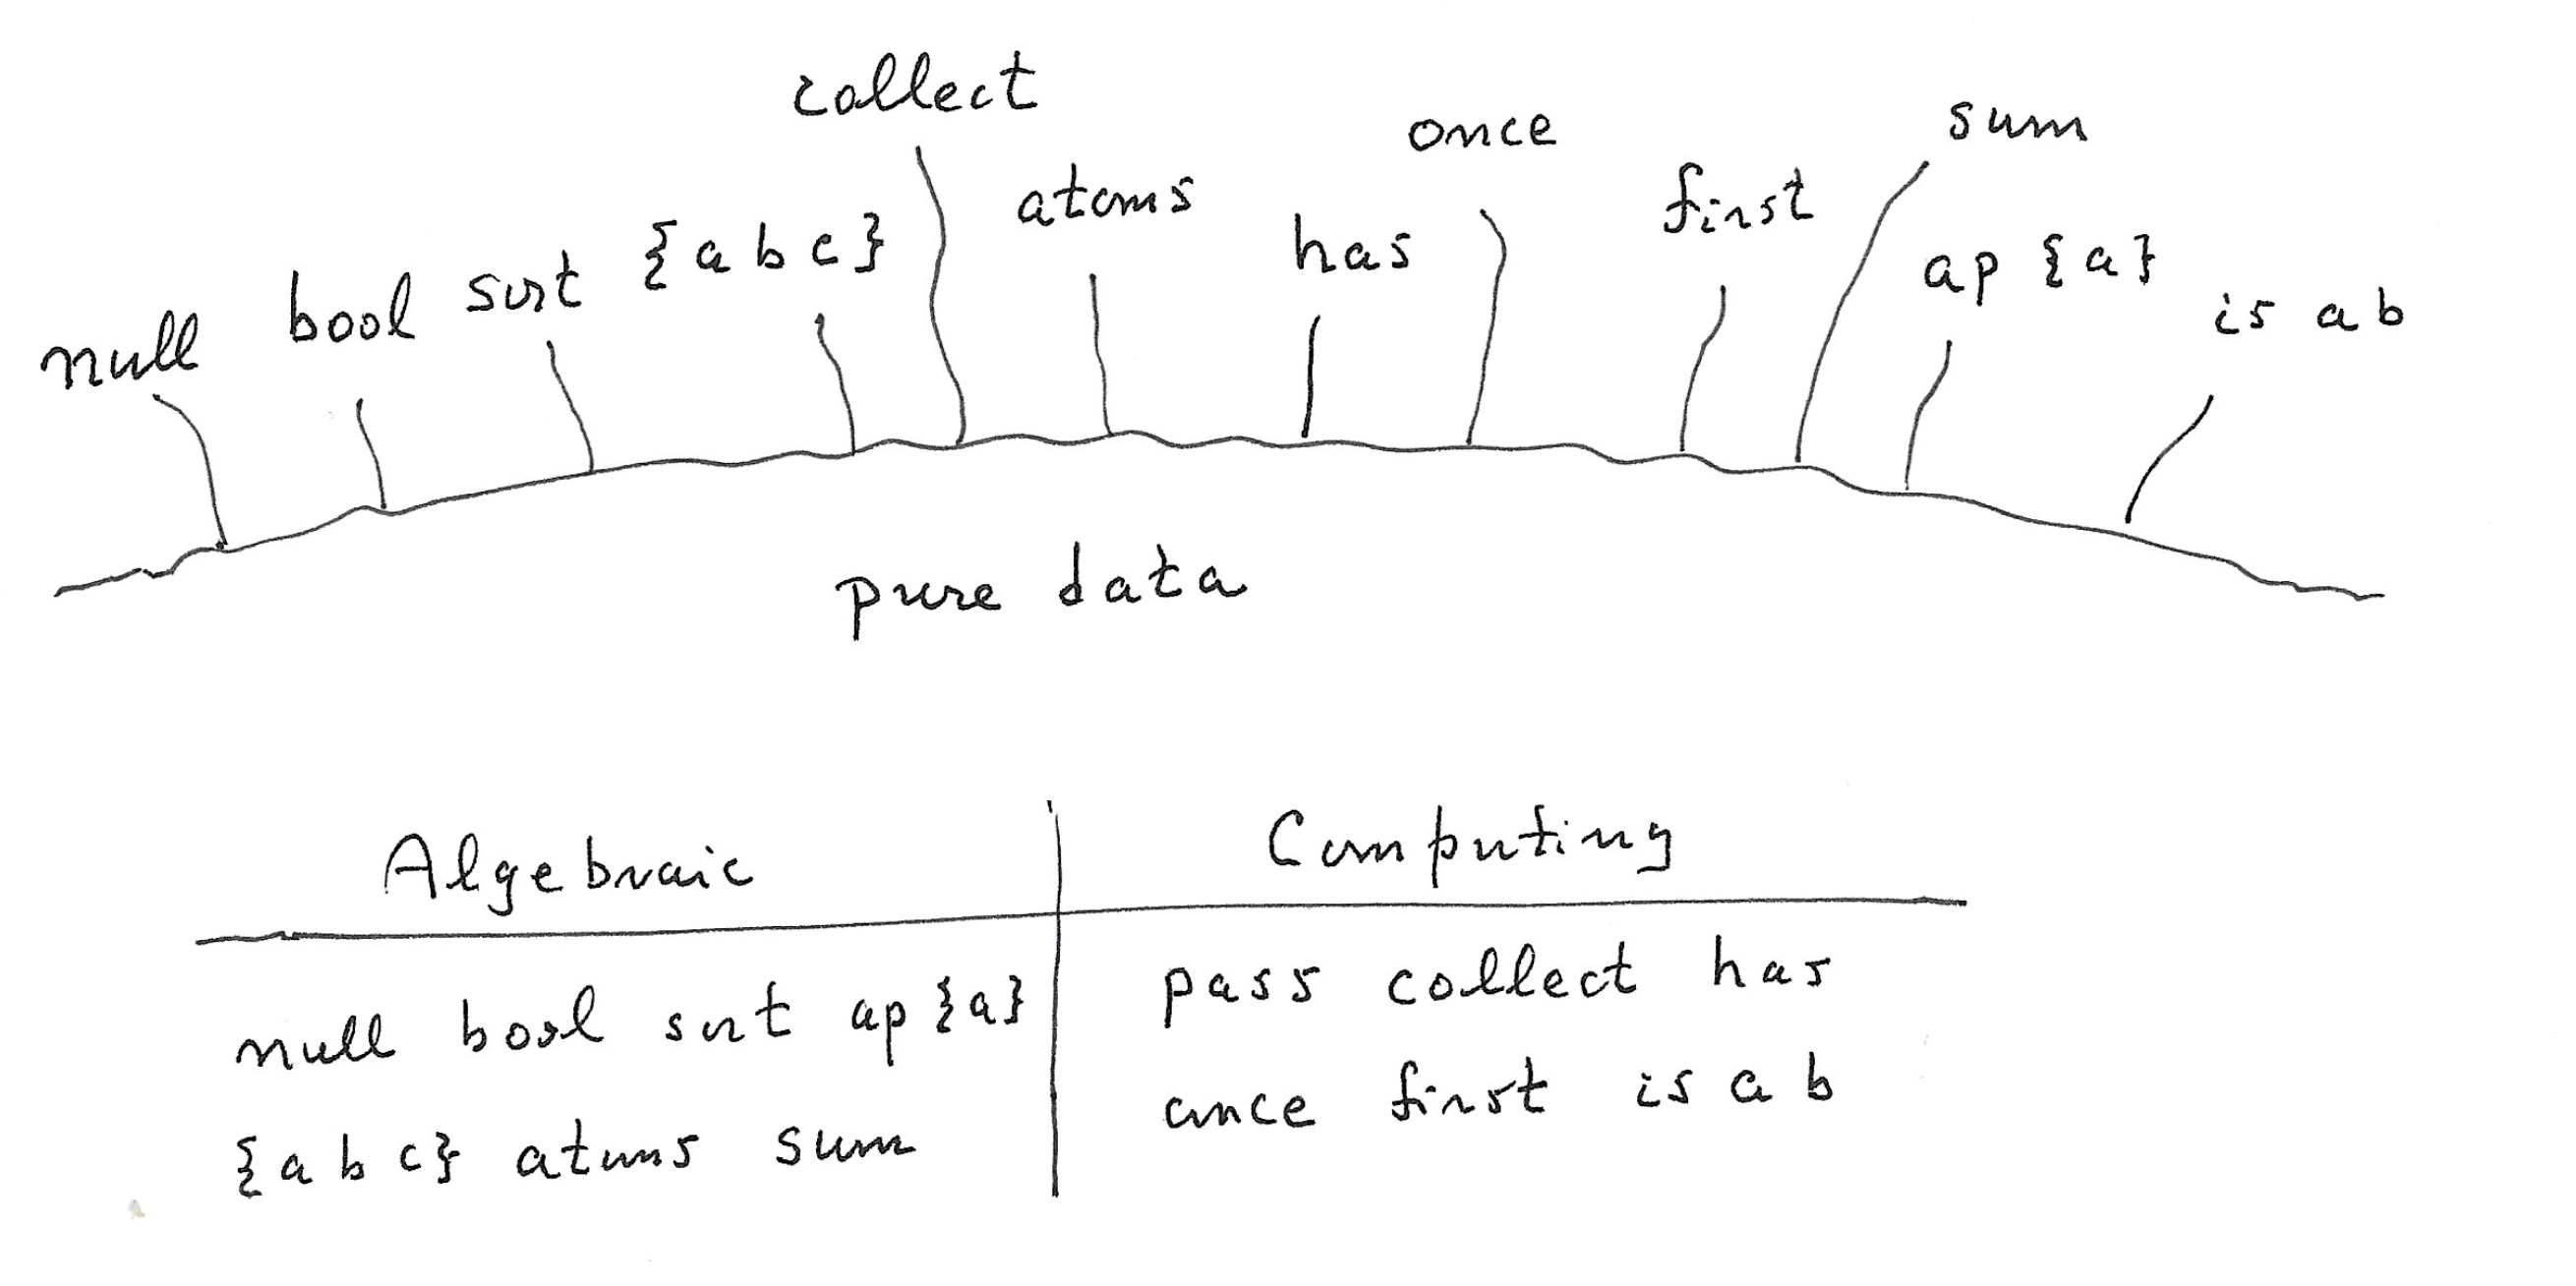
\includegraphics[width=0.8\textwidth]{garden1.png}
\caption{{\it The space of all pure data contains all mathematical objects.  Our strategy for exploring this space is to first introduce 
the minimal combinatorics implicit from the foundational finite sequence concept, and then examine the simplest spaces first as they 
appear ``organically.''  Since algebraic spaces are commutative, they, in a sense, transcend the foundational sequence concept and are more ``Platonic.''}}
\end{figure}

\section{The Space of all data} 

     As a first example and for orientation, let's consider the space of all pure data.  Since (pass:X)=X for all data X, the distributive space pass 
contains all pure data.  Since spaces are fixed points on their contents, pass is the unique space containing all data.  Every data $X$ is both in pass
and is also an endomorphism of pass, since $X$ is equal to pass$\cdot X\cdot$pass.  Thus, the semiring of pass is also the collection of all data, with 
addition ($X\oplus Y$)=($X+Y$), and multiplication $(X\cdot Y)$.  The units of the semiring are $1$=pass$\cdot$pass$\cdot$pass=pass, 
and $0$=pass$\cdot$null$\cdot$pass=null respectively.   

Consider the properties defined in section 6.  
\begin{itemize}
\item{{\bf Subspaces.}  Since every data is a morphism of pass, every space is a subspace of pass.  The constants of pass are the data $K$ such that 
$K\cdot 0$=$K$, in other words, the constant spaces (const $K$) are the constants.}
\item{{\bf Homomorphisms.} Since pass is distributive, the homomorphisms of pass are the distributive data in pass, including spaces, such as (ap \{a\}) 
and non-spaces such as (ap \{B B\}).} 
\item{{\bf Group of units.} The units of pass are permutations such as (swap 1 2) and (rev).  The central constants of pass are the data which 
are invariant under all permutations.  These are the sequences of identical atoms such as (:) (:) (:) or (a a a a a).  These can be interpreted as ``organic natural numbers.''}
\item{{\bf Central endomorphisms} The maximally platonic, maximally significant content of pass are the central homomorphisms, which include 
subspaces such as (ap const a), (atoms), (is b).  These are isomorphic spaces, each representing natural numbers with natural number 
addition.  This and the direct connection of bool with the underlying pure data context means that 
both the natural numbers and bool are good starting points for exploration.} 
\item{{\bf Semialgebra} In pass, there is a bijection between the homomorphisms of pass and the constants of pass given by $X\leftrightarrow ({\rm ap}\ X)$.  Thus,
pass is a semialgebra as well as a semiring with $X\star (Y+Z)$ equal to $(X\star Y)+(X\star Z)$ where $X\star Y$ is defined to be (ap $X$)$\cdot Y$.}
\item{{\bf Semilattice} The ideal semilattice includes the spaces (bool), (once) and (const $K$) for any data $K$. Although not a homomorphism,
bool is a central endomorphism as well as a semilattice and is the unique space with exactly two fixed points.} 
\item{{\bf Idempotents} The idempotent equivalence classes of pass includes all idempotent data where (pass) is the unique maximum idempotent and where all constants 
are in the minimal equivalence class.}
\end{itemize}
In the idempotence order, pass is the unique maximum $X{\overset i\leq}{\rm pass}$ since pass uniquely satisfies 
$X\cdot {\rm pass}=X$ for all $X$.  Pass is its own image and the kernel of pass is the maximal idempotent $e$ such that $e\cdot {\rm pass}={\rm null}\cdot{\rm pass}$, 
so the space (null) is the kernel of pass.  

\begin{figure}[h]
\centering
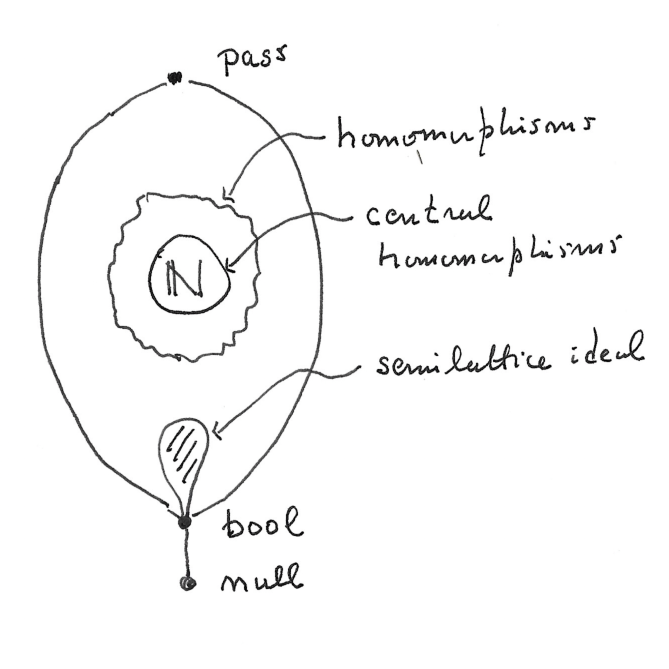
\includegraphics[width=0.6\textwidth]{pass.pdf}
\caption{{\it As a collection, pass contains all pure data; that is, all objects with mathematical 
meaning as well as all computations.  As a space, it has a specific structure which is typical of other examples in the text.  
In the idempotent partial order, (pass) is the unique maximum and (null) is minimal.  Each data in pass is also an endomorphism of pass.  The homomorphisms of pass are the distributive data.  The central homomorphisms are a single isomorphism class equivalent to the ``organic'' natural 
numbers.  Spaces that are fields includes bool, null, and the rem(p,p) subspaces of ${\mathbf N}$, equal to ${\mathbf F}_p$ for prime $p$.  Bool and null are in the ideal of semilattice spaces as well.}}
\end{figure}

In classical mathematics, the concept of a Set intentionally gives no information about its contents.  Thus, the ``Set of all Sets" is vast and, in 
a sense, contains everything, but we don't expect any insight from this.  The space (pass) is also vast.  It contains all mathematical objects 
of any kind and all possible computations within the framework of pure data.  Nevertheless, pass does have a specific structure with specific 
features that indicate what is most important mathematically: the central homomorphisms (the natural numbers) and the central semilattice (bool).  
After describing (pass) and (null), these will be our starting points for investigation.  

\section{Null}

    Null is the distributive algebraic space defined by (null:$X$)=() for all $X$.  Since null$\cdot X\cdot$null=null, null is the only endomorphism 
of null, and so 1=0 in the semiring, as is true for all other constant spaces.  Since $0\cdot(0\oplus 0)=(0\cdot 0) \oplus (0\cdot 0)=0$, the one 
endomorphism is a homomorphism as well as a subspace. 
Null is minimal in the idempotence order, as is all of the 
other constant spaces.  The kernel of null is pass.  

\section{Organic Numbers}

      We have seen that ``organic natural numbers'' appear as sequences of identical atoms where we identify (:) (:) (:) or (a a a) with ``3,'' just depending 
 on a conventional choice of atom to represent ``1.''  The spaces where these numbers are data are the maximally platonic central homomorphisms of 
 pass.  For instance, the spaces (atoms), (ap const (:)), (ap const a), (ap \{\#\}), (is a) all are central homomorphisms and each represents natural numbers 
 with natural number addition.  Since these spaces are isomorphic and, therefore, have the same semirings, we can choose any one for investigation.  
 For convenience we will choose (is a) as the particular space to start with.  For convenience, denote n concatenations of data $A$ by $A^n$ so so that 
 ``5'' represented by (a a a a a) and can be written as a$^5$.  The space (is a) has natural extensions (is a b), (is a b c),$\dots$.  
 Lets agree to denotes these spaces by $N_1$, $N_2$, $N_3\dots$ and refer to these spaces and their subspaces as the ``organic numbers.'' 
      
\subsection{Organic Natural Numbers}     
     
     The first thing to notice is that $N_1$ contains one data a$^n$ for each natural number $n$, and addition in $N_1$ is natural number addition, 
since ($N_1$:$X$\ $Y$) is the natural number sum of ($N_1$:$X$) and ($N_1$:$Y$).  Since homomorphisms are distributive, a homomorphism $h$ of $N_1$ is determined by ($h$:a), so that $h$ is natural number multiplication by some natural number, 
for instance, ($h$ = ap const a\ a\ a) is multiplication by $3$.  There is one such homomorphism for each data in $N_1$, and so $N_1$ is a semialgebra and 
is identical to the standard semiring of natural numbers with multiplication distributing over addition.
     
    Subspaces of $N_1$ are indicated by subspace endomorphisms.  As always, the subspace $1$ is the whole of $N_1$ and the subspace $0$ consists of just the neutral data of $N_1$, which, 
since $N_1$ is distributive, is the empty sequence.  It is easy to guess some subspaces of $N_1$.
\begin{itemize} 
\item [1.] {\bf Saturation subspaces} An endomorphism (min a a) is a subspace which effectively computes the minimum of 2 and its argument.  Thus (min a a) contains the data (), (a), and (a a). 
\item [2.] {\bf Modular arithmetic subspaces} An endomorphism which removes three (a) atoms while possible, such as (while remove a a a) is a subspace which computes the sum modulo 3.  Note 
that (while remove a a a) contains the same data as (min a a), but they have a completely different algebraic structure.  
\end{itemize}
These unsurprising subspaces have a slightly more surprising generalization.  For $p,q\ge 1$, let rem($p$,$q$) be the endomorphism defined by 
\begin{equation}
{\rm while}\ n\ge p,q: {\rm remove\ p\ from\ n}
\end{equation}
The rem(p,q) are also subspaces and modular sum and saturation cases since rem($p$,$p$) is $n\mapsto n$ mod $p$ and rem($1$,$q$) is $n\mapsto$ min($n$,$q-1$).   The rem subspaces are also closed under composition via 
\begin{equation}
{\rm rem}(p,q)\cdot {\rm rem}(p',q') = {\rm rem}({\rm LCM}(p,p'),{\rm max}(q,q'))
\end{equation}
where {\it LCM} is the least common multiple.  This makes the rem a closed commutative semilattice of subspaces of $N_1$.  

\begin{figure}[h]
\centering
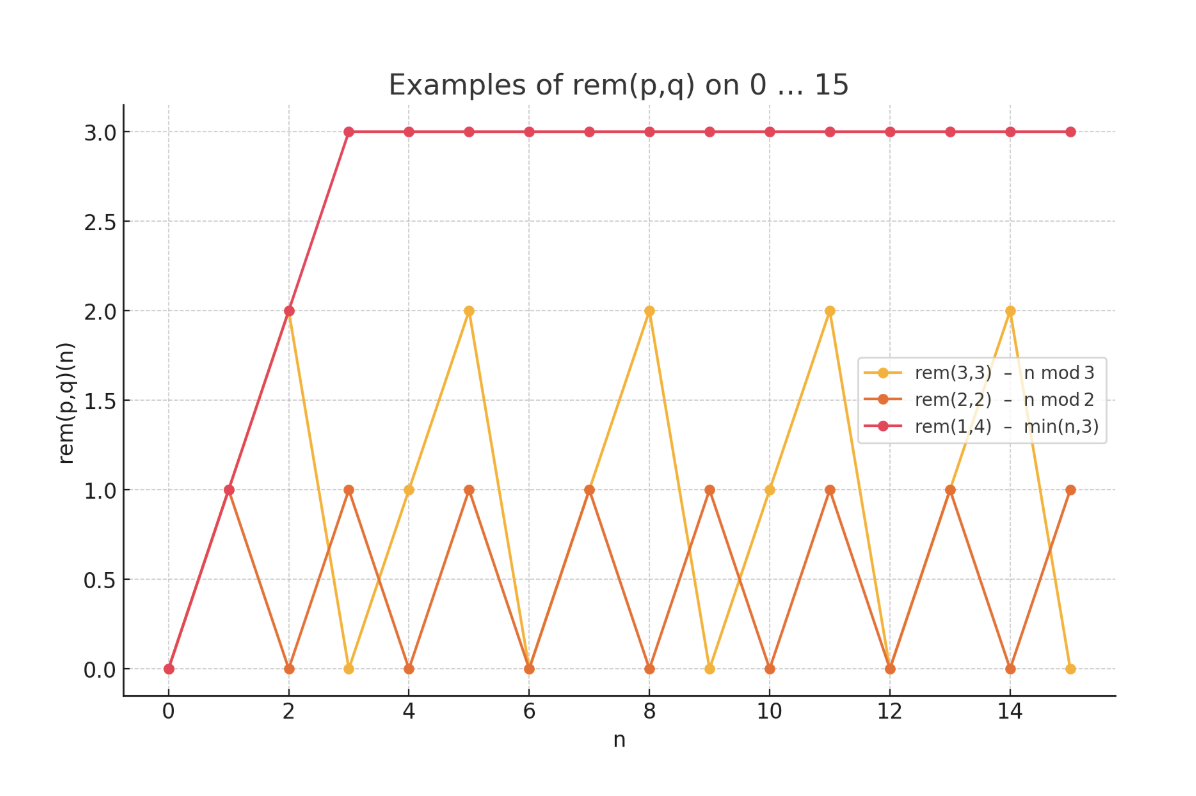
\includegraphics[width=0.7\textwidth]{rem.png}
\caption{{\it Subspaces of (is a) or $N_1$ are N, constants and rem(p,q) subspaces.  These specialize to natural numbers mod p and ceiling functions min(q).}}
\end{figure}

This completes the analysis of $N_1$.  The homomorphisms of $N_1$ are multiplication by natural numbers, making $N_1$ a semialgebra 
identical to the standard semiring $\mathbb N$.  The subspaces of $N_1$ are 1, the constants and the rem(p,q) subspaces.  All subspaces 
are mutually commuting and, thus, are closed under composition.  

\begin{proof}
Let $f:{\mathbf N}\rightarrow{\mathbf N}$ where $f(x+y)=f(f(x)+y)=f(x+f(y))$ for all $x,y\in\mathbf N$...
\end{proof}

\subsection{is a b} 

The second simplest ``organic number'' is (is a b), which we can refer to as N$_2$ for brevity.  Since N$_2$ is distributive, the homomorphisms of N$_2$ 
are the distributive endomorphisms.  Consider subspaces N$_2$.  

\begin{itemize}
\item{The subspaces 1 and 0 give the whole of N$_2$ and just the empty sequence as subspaces, respectively.  
Projections N$_2$$\cdot$(is a)$\cdot$N$_2$ and N$_2$$\cdot$(is b)$\cdot$N$_2$ produce two N$_1$-isomorphic subspaces.}

\item{Let `reduce' be the endomorphism of N$_2$ which removes (a b) and (b a) subsequences until saturation.  Thus, every data in reduce
is either a$^n$ or b$^n$ for some natural number $n$.  A homomorphism $h$ satisfies $h:X\ Y$ = reduce $:(h:X)\ (h:Y)$, so 
$h$ is determined by ($h$:a) and ($h$:b).  If $h$ is a central homomorphism, ($h$:b) is ($h$:a) followed by an 
a$\leftrightarrow$b swap.  Thus, if we interpret a$^n$ as the integer $n$ and b$^n$ as the integer $-n$, then applying $h$ 
is standard distributive integer multiplication by the integer ($h$:a).  Since there is one central homomorphism for each data in the subspace reduce, 
reduce is a central semialgebra isomorphic to the standard ring $\mathbf Z$ of integers.}

\item{If `sort' is the endomorphism which does lexical sorting of N$_2$ data, then sort is also a subspace of N$_2$ where the 
data of sort can be written $a^m b^n$ for $m,n\ge 0$.  As in the previous case, a homomorphism M of sort is defined by  
\begin{itemize}
\item [] $M: a\mapsto a^{m_{11}} b^{m_{21}}$, and 
\item [] $M: b\mapsto a^{m_{12}} b^{m_{22}}$ 
\end{itemize}
for some choice of 
$
\left (
\begin{array}{cc} 
m_{11} & m_{21} \\ m_{12} & m_{22}  
\end{array}
\right ) 
$
so the action of M is standard matrix multiplication.  Thus, the data of sort are pairs of natural numbers and the 
homomorphisms are 2x2 matrices with natural number entries.  The central homomorphisms of sort 
commute with the involution 
$
\left (
\begin{array}{cc} 
0 & 1 \\ 1 & 0 
\end{array}
\right ) 
$
and so the central homomorphisms are matrices 
$
\left (
\begin{array}{cc} 
m & n \\ n & m 
\end{array}
\right ) 
$
for natural numbers $m$ and $n$.  Thus, there is exactly one central homomorphism for each data in sort, 
and sort is, therefore, a central semialgebra, equivalent to the standard matrix semiring ${\rm Mat}_{2\times2}(\mathbf N)$.
}

\item{Lexical sort followed by reducing (b b) to (b) results in a subspace equivalent to $\mathbf N\times\{0,1\}$ with addition
defined by $(n,\alpha)+(m,\beta)$=$(n+m,\alpha\vee\beta)$.}

\item{Lexical sort followed by reducing $a^n b^m$ to $a^{(n/g)} b^{(m/g)}$ where $g$=GCD$(n,m)$ is the greatest common divisor.  
This is the space of positive rational numbers, but with non-standard `mediant' addition[ref].}

\end{itemize}

\subsection{xxxx} 

     It is clear that in going to higher organic numbers, some of the features of $N_1$ and $N_2$ will repeat.  $N_n$ sorted 
 will always result in a space with homomorphisms ${\rm Mat}_{n\times n}(\mathbf N)$.  Sorting followed by cancelling 
 atoms in pairs will result in ${\rm Mat}_{(n/2)\times (n/2)}(\mathbf Z)$
 
 Examples...
 \begin{itemize}
 \item{In $N_4$=(is a b c d), with (a b)=(b a)=(c d)=(d c)=(), the homomorphisms are all of ${\rm Mat}_{2\times 2}(\mathbf Z)$.  The 
 central homomorphisms, however, must commute with 
 $
J=
\left (
\begin{array}{cc} 
0 & -1 \\ 1 & 0 
\end{array}
\right ) 
$
and are thus 
$
\left (
\begin{array}{cc} 
a & -b \\ b & a 
\end{array}
\right ) 
$
so the central homomorphisms of $N_4$ is a central semialgebra equivalent to the Gaussian integers ${\mathbf Z}[i]$.
}

\item{Quaternions}
\item{Octonions, even though semirings ops are associative}  
\end{itemize} 

\begin{figure}[h]
\centering
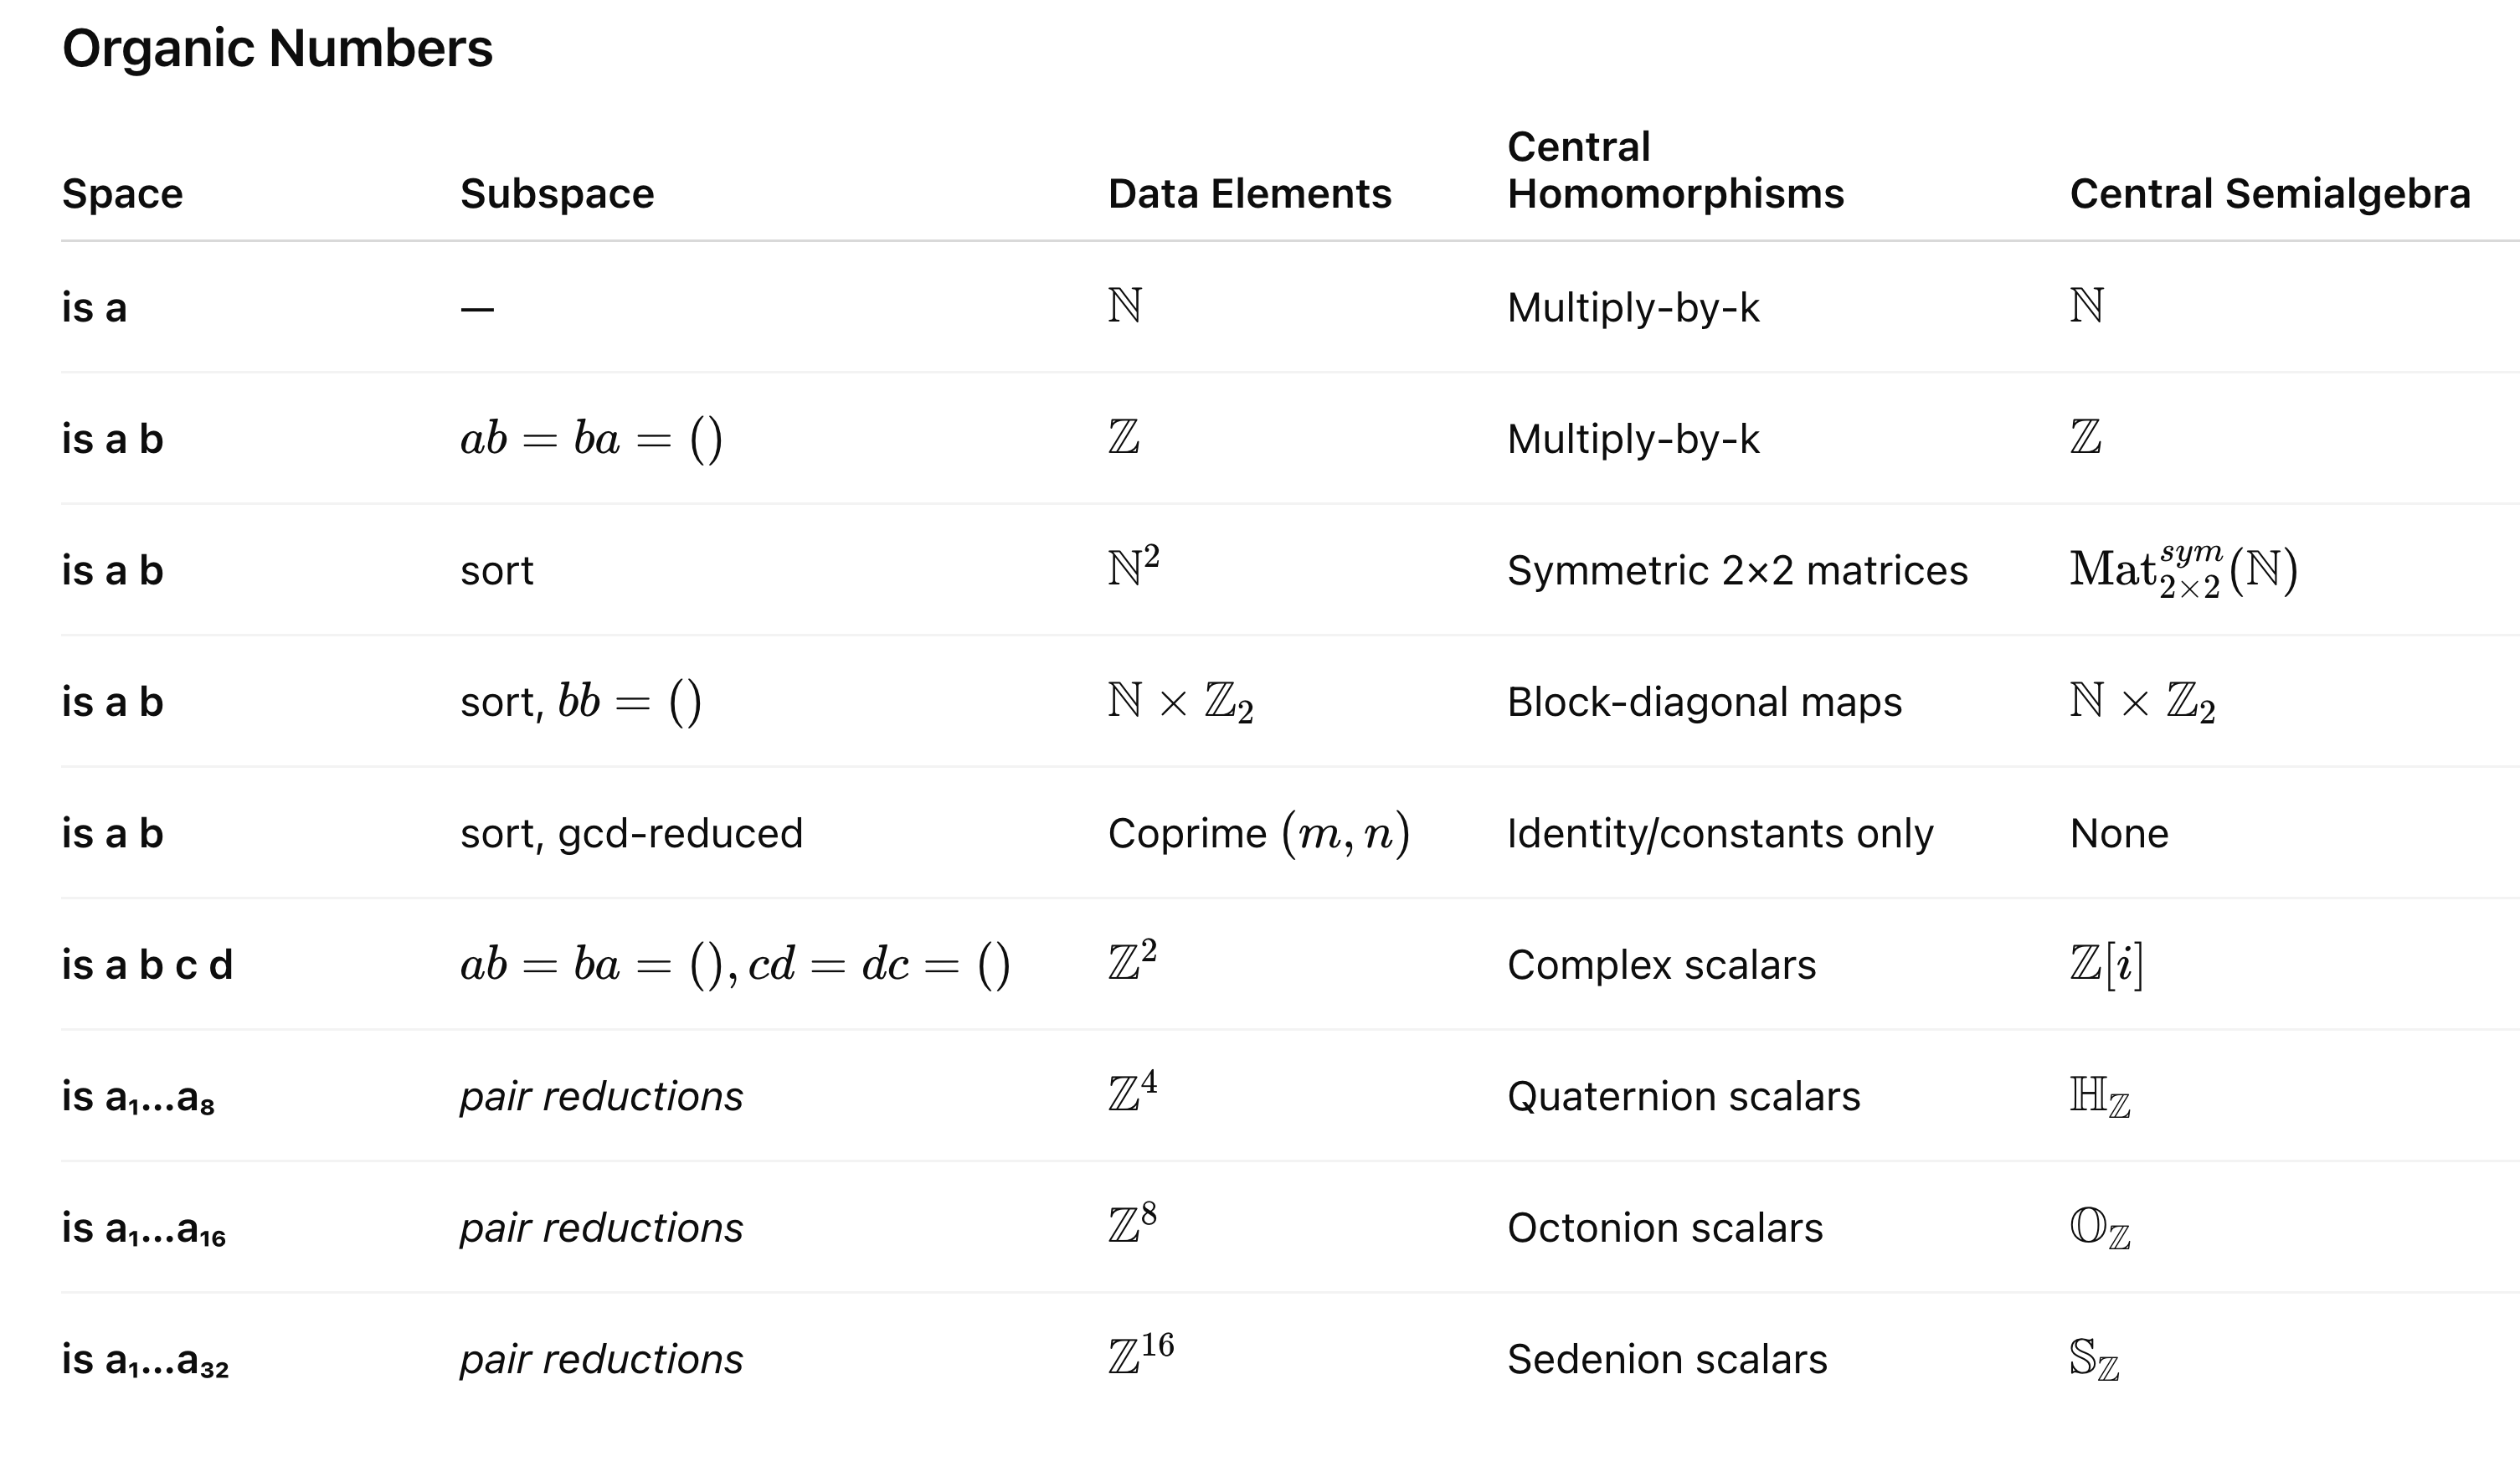
\includegraphics[width=1.0\textwidth]{OrganicTable.png}
\caption{{\it Organic Numbers.}}
\end{figure}

\subsection{Number Sequences}

      Given the space $N_1$ from the previous section, let $\mathbb{N}$ be 
\begin{equation}
{{\rm ap}\ ({\rm put\ {\rm n}})\cdot N_1 \cdot ({\rm get\ {\rm n}})}
\end{equation}
where `n' is some chosen atom.  Since $({\rm put\ n})\cdot N_1 \cdot ({\rm get\ n})$ is idempotent, ${\mathbb N}$ is a distributive space containing 
sequences of $n$-atoms containing $N_1$-data, such as 
\begin{equation} 
{\rm T = (n:a\ a\ a)\ (n:)\ (n:a\ a)\ (n:a)\ (n:)}
\end{equation} 

Unlike the case of $N_1$, the action of ${\mathbb N}$ is merely to concatenate sequences.  It's easy, however, to identify 
natural number sum again as one of several subspaces 
\begin{itemize}
\item sum:T = (n:a a a a a a)
\item sort:T = (n:) (n:) (n:a) (n:a a) (n:a a a)
\item min:T = (n:)
\item first:T = (n:a a a)
\end{itemize} 
All but the last are algebraic subspaces and, predictably, have established names.  
Some endomorphisms of ${\mathbb N}$ are ``inherited'' from $N_1$ as follows.  Define inner:F to be 
\begin{equation}
{\mathbb N}\cdot({\rm put\ n})\cdot {\rm F}\cdot({\rm get\ n})\cdot{\mathbb N}
\end{equation}
so that (inner:F):X means letting F act on the concatenated $N_1$-contents of $X$, returning the result in a single n-atom.  The sum endomorphism 
above, for instance, is equal to inner:$N_1$.  The construction of Equation 7 works for any space, and so we can define a ``functor'' {\it Seq} to be 
\begin{equation}
\{({\rm put}\ {\rm A})\cdot {\rm B} \cdot ({\rm get}\ {\rm A})\}
\end{equation}
Then {$\mathbb N$} is equal to (Seq n:$N_1$) and given any atom s and any space S, (Seq s:S) is the space of S-values stored in s-atoms.  
Similarly, if we define {\it inner} to be  
\begin{equation}
S\cdot\{({\rm put\ s})\cdot{\rm B}\cdot({\rm get\ s})\}\cdot S
\end{equation}
then inner:$f$ is the inner version of an endomorphism $f$ of $S$.  Other general constructions of this type are possible.  For example, 
since the endomorphism last2 = (inner:last 2) sums the last two atoms of a data of ${\mathbb N}$, (series last2) generates the fibonacci sequence. 

\begin{figure}[h]
\centering
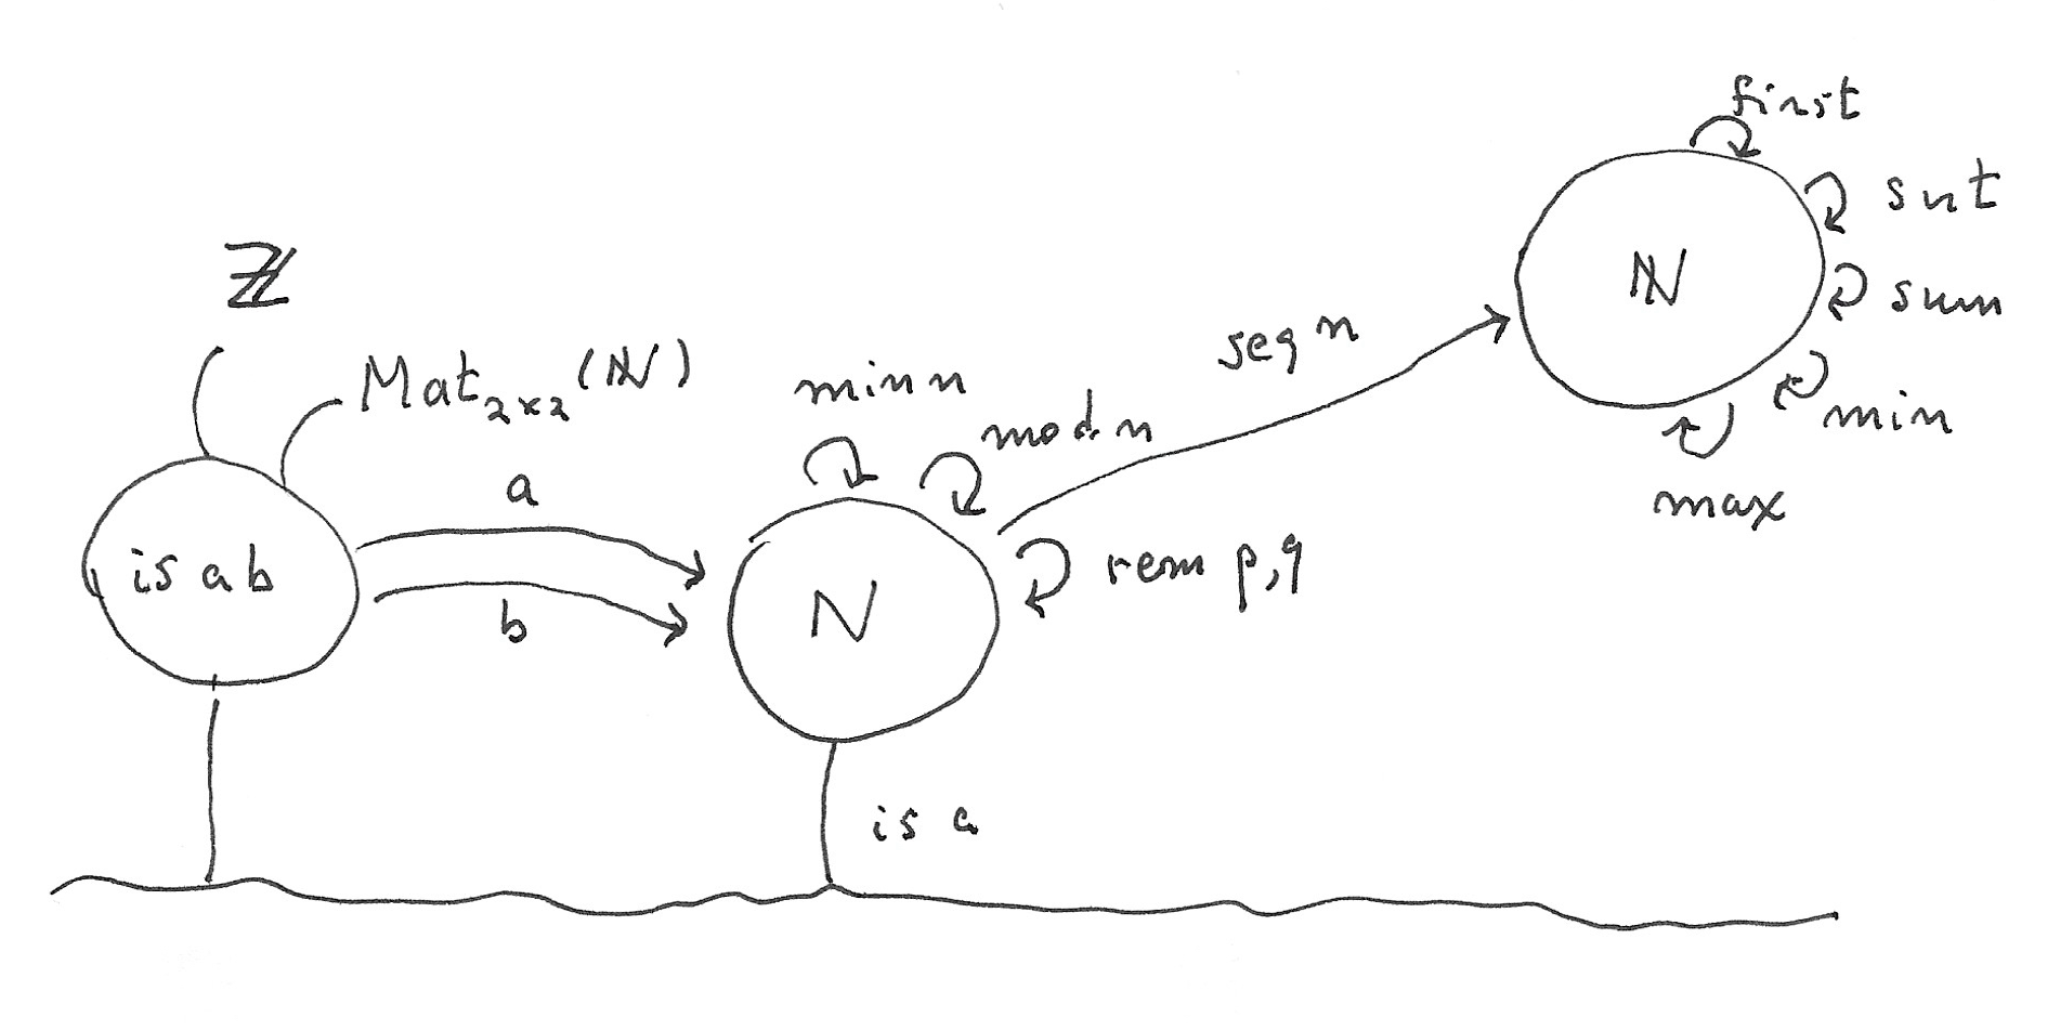
\includegraphics[width=0.7\textwidth]{organics.png}
\caption{{\it Organic numbers.}}
\end{figure}


\section{Boolean} 

      As mentioned already, the space bool is likely to be mathematically interesting, both because of its direct connection to 
the underlying pure data context and, in abstract terms, because it is a central, algebraic space within pass.  Although central, bool is not a 
homomorphism and so has a different character from natural numbers.  
Since bool contains two data:  () for {\it true} and (:) for {\it false}, bool has only four endomorphisms:  
the identity ID=bool, two constants: TRUE=(const ()), and FALSE=(const (:)), and one involution NOT=bool$\cdot$not$\cdot$bool.  
Since there are only four, we include the complete semiring operations in Table X.  Note that $\oplus$ is commutative since 
bool is algebraic and $f\oplus f=f$, since bool has the semilattice property.  
\begin{table}
\begin{tabular}{| l | l | l | l | l |  }
$f\cdot g$ & ID & TRUE & FALSE & NOT  \\
\hline
ID &  ID & TRUE & FALSE &  NOT \\
TRUE & TRUE & TRUE  & TRUE & TRUE \\
FALSE & FALSE  & FALSE & FALSE & FALSE   \\
NOT & NOT & FALSE & TRUE & ID \\
\hline
\end{tabular}
\begin{tabular}{| l | l | l | l | l |  }
$f\oplus g$ & ID & TRUE & FALSE & NOT  \\
\hline
ID &  ID & ID & FALSE & FALSE \\
TRUE & ID & TRUE  & FALSE & NOT \\
FALSE & FALSE  & FALSE & FALSE & FALSE   \\
NOT & FALSE & NOT & FALSE & NOT \\
\hline
\end{tabular}
\caption{{\it Product and sum of the four morphisms ID, TRUE, FALSE, NOT of the space bool}.  Note that ID is the unit of multiplication and TRUE is the 
unit of addition, and we have $f\oplus g=g\oplus f$, since bool is algebraic, and $f\oplus f=f$.}
\end{table}
The subspaces of bool are ID, TRUE and FALSE, so bool has only trivial subspaces.  The endomorphisms ID and TRUE are neutral, ID is the only positive 
endomorphism and all endomorphisms are algebraic since bool itself is algebraic.  The group of units is ID and NOT, and ID is the only central endomorphism. 

\subsection{Boolean Sequences}

As in the case of N, we can let $\mathbb L$=(Seq b:bool), be the distributive space of bool-valued data stored in b-atoms, so a typical data in $\mathbb L$ is 
\begin{equation}
{\rm (b:)\ (b:)\ (b:(:))\ (b:)\ (b:(:))\ (b:(:))}
\end{equation}
Let's agree to write such sequences replacing (b:) with T, (b:(:)) with F and the empty sequence with 0, so that the above is written TTFTFF.   
Let's also consider the shortest subspaces of $\mathbb L$ first.  
The subspace ${\mathbb L}\cdot {\rm first}\cdot{\mathbb L}$ contains the $\mathbb L$ sequences of length less than or equal to 1 and similarly,  
${\mathbb L}\cdot {\rm first\ 2}\cdot{\mathbb L}$ is the subspace of sequences with length less than or equal to 2.  Lets refer to these spaces as 
${\mathbb L}_1$ and ${\mathbb L}_2$ repectively.  
Thus, ${\mathbb L}_1$ contains data \{0,T,F\} and ${\mathbb L}_2$ contains data \{0,T,F,TT,TF,FT,FF\}. 
For ${\mathbb L}_1$, we can specify an endomorphism $f$ of ${\mathbb L}_1$ by listing the values of $f$ on 0,T,F in standard order.  So, for example, 
`0TF' denotes the identity endmorphism of ${\mathbb L}_1$.  
Since ${\mathbb L}_1$ has 27 morphisms, we can be completely explicit about this space.  
Figure 4 lists the 27 endomorphisms and indicates endomorphisms with special properties.  Even with relatively small space like ${\mathbb L}_1$, all of 
the classes of endomorphisms appear in a nontrivial way.

\begin{figure}[h]
\centering
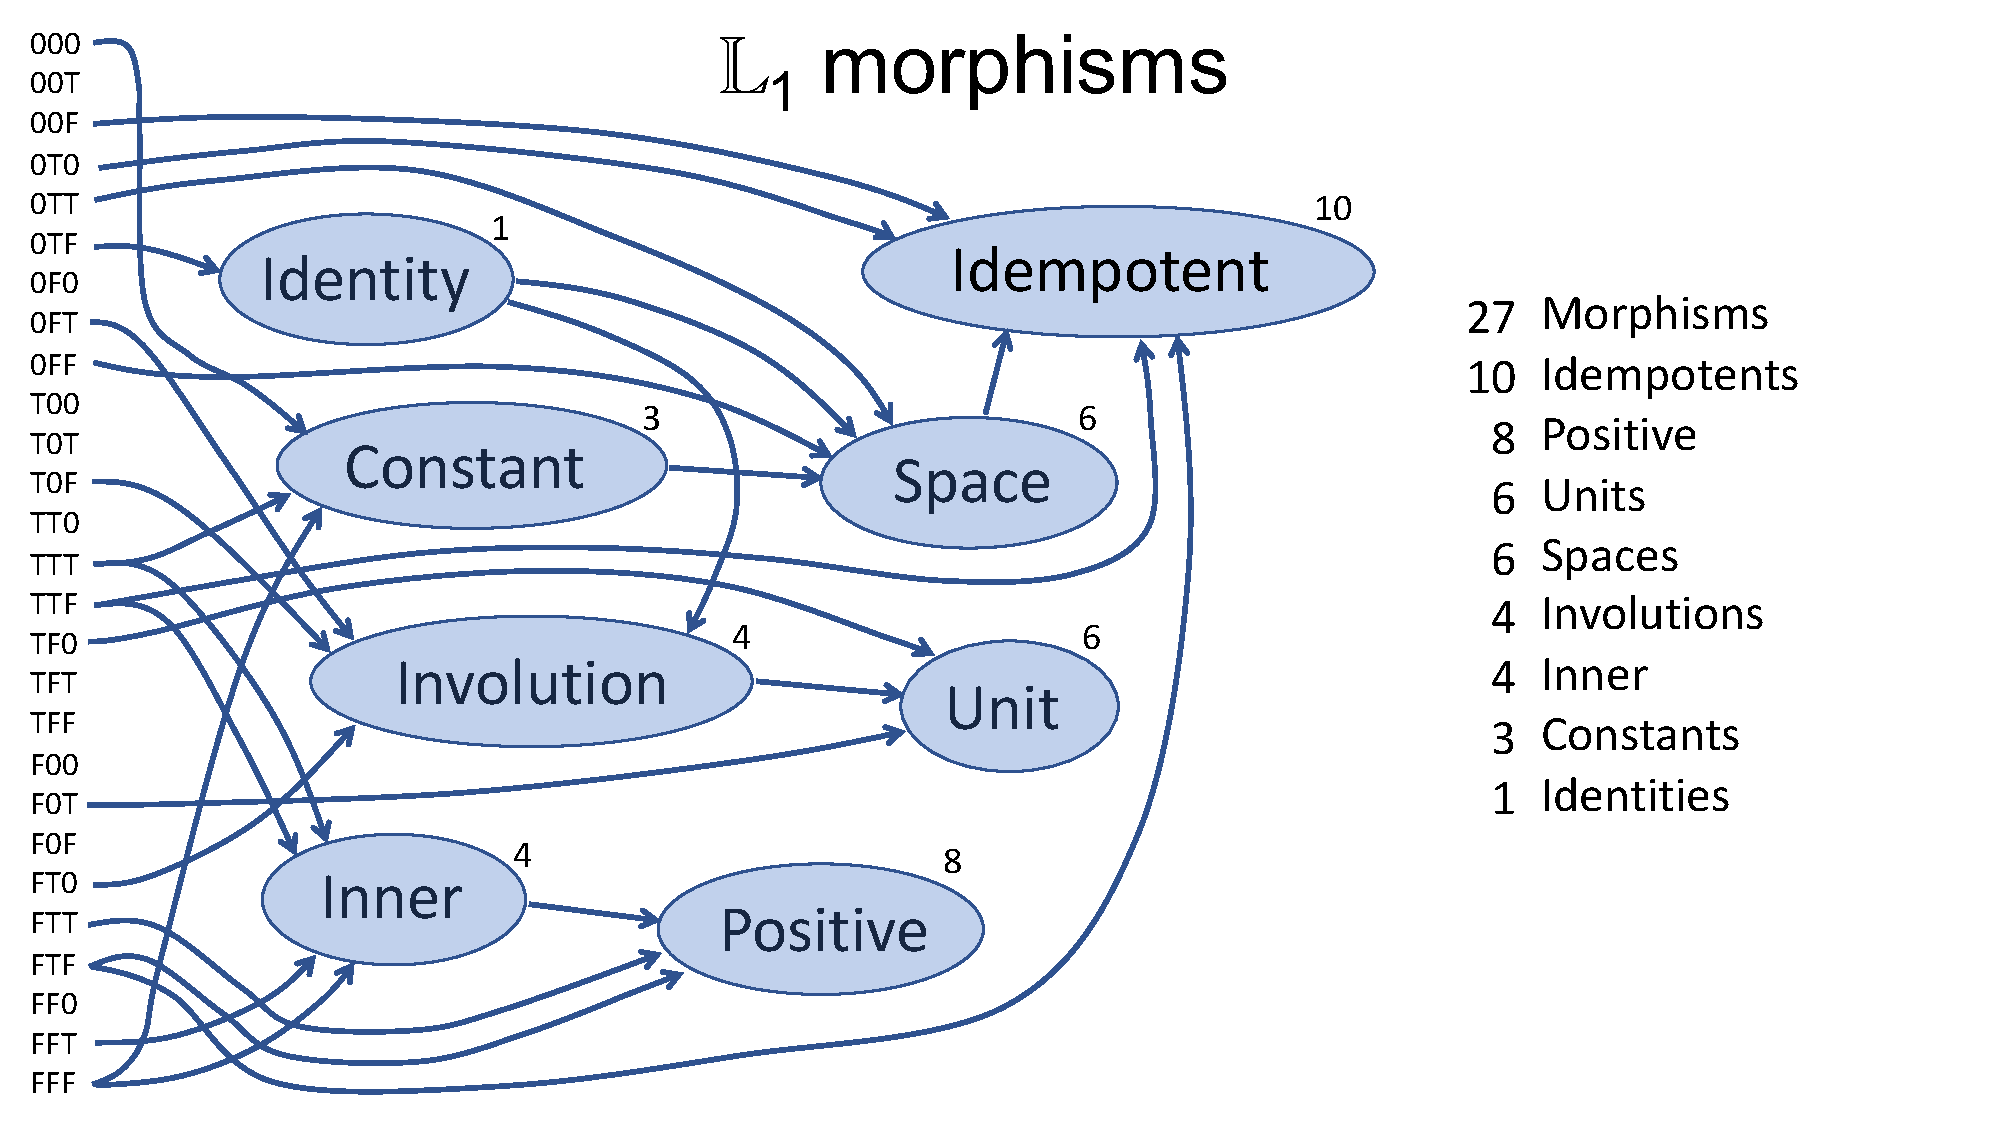
\includegraphics[width=0.8\textwidth]{L1.pdf}
\caption{{\it The endomorphisms of ${\mathbb L}_1$ are maps from from \{0,T,F\} to itself. These are specified as the three function 
values in the column on the left.  Even with a small space of this size, the $3^3=27$ all of the classes of endomorphism identified in the text 
appear in a non-trivial way.}}
\end{figure}

    Moving to ${\mathbb L}_2$, there are already $7^7=823,543$ morphisms; far too many to be as explicit as in the case of ${\mathbb L}_1$.  
 As a first attempt, examine just the inner endomorphisms, since there are only eight of these consisting of 
 the endomorphisms ${\mathbb L}_2\cdot ({\rm put}\ b)\cdot {\rm F} \cdot ({\rm get}\ b) \cdot {\mathbb L}_2$
for some data $F$.  These eight depend only on the total number of (:) values in the b-atoms of input, and each morphism returns exactly one b-atom.  
The inner morphisms of ${\mathbb L}_2$ are all central homomorphisms, so we might expect them to be
mathematically interesting.   
\begin{table}
\caption{The eight inner morphisms of ${\mathbb L}_2$ slightly generalize the eight standard symmetric binary boolean operators.}
\centering 
\begin{tabular}{r c c c c c c c r r l}
\hline\hline
$e_i \in {\mathbb L}_2$ & 0 & T & F & TT & TF & FT & FF & standard & generalized & description \\ [0.5ex] 
\hline
$e_1$  & T & T & T & T & T & T & T & TRUE & {\bf always} & always true \\
$e_2$  & T & T & T & T & T & T & F & OR & {\bf any} & any are true \\
$e_3$  & T & T & F & T & F & F & T & XNOR & {\bf even} & even (:)s \\
$e_4$ & T & T & F & T & F & F & F & AND & {\bf all} & all are true \\
$e_5$ & F & F & T & F & T & T & T & NAND & {\bf notall} & not all are true \\
$e_6$ & F & F & T & F & T & T & F & XOR & {\bf odd} & odd (:)s \\
$e_7$ & F & F & F & F & F & F & T & NOR & {\bf none} & none are true  \\
$e_8$ & F & F & F & F & F & F & F & FALSE & {\bf never} & never true \\
\hline
Number of (:)   & 0 & 0 & 1 & 0 & 1 & 1 & 2 &  \\ 
\hline
\end{tabular}
\label{table:L2}
\end{table} 
Indeed, Table Y shows the eight morphisms and their values on \{0,T,F,TT,TF,FT,FF\}.  Looking at the values for the last four entries \{TT,TF,FT,FF\} 
we recognize that these are slight generalizations of the eight standard symmetric binary boolean operators.  The values of the eight morphisms 
on \{0,T,F\} suggests that the standard binary operator names (`OR' as opposed to `any') are not particularly illuminating in this larger context.  

\section{Summary, Global Strategies, Questions} 

Summary:  we have a coherent view of mathematics analogous to sets with structure or Category Theory.  
\begin{itemize}
\item{View as pure data, semiring or confluent sequence compatible rewrites within a global rewrite.  Pure data is good for searching ordered by "organic".  
semiring is good for adapting math ideas from semiring, near-ring, theory etc.  Rewrite may provide a way to generalize from the underlying space 
of all pure data.} 
\item{Deeper results, algebra, geometric constructions, Homotopy,...} 
\item{Use deep learning to treat evaluation like a game to be learned.  Automating, searching, proofs, optimizing computations.} 
\end{itemize}


\begin{figure}[h]
\centering
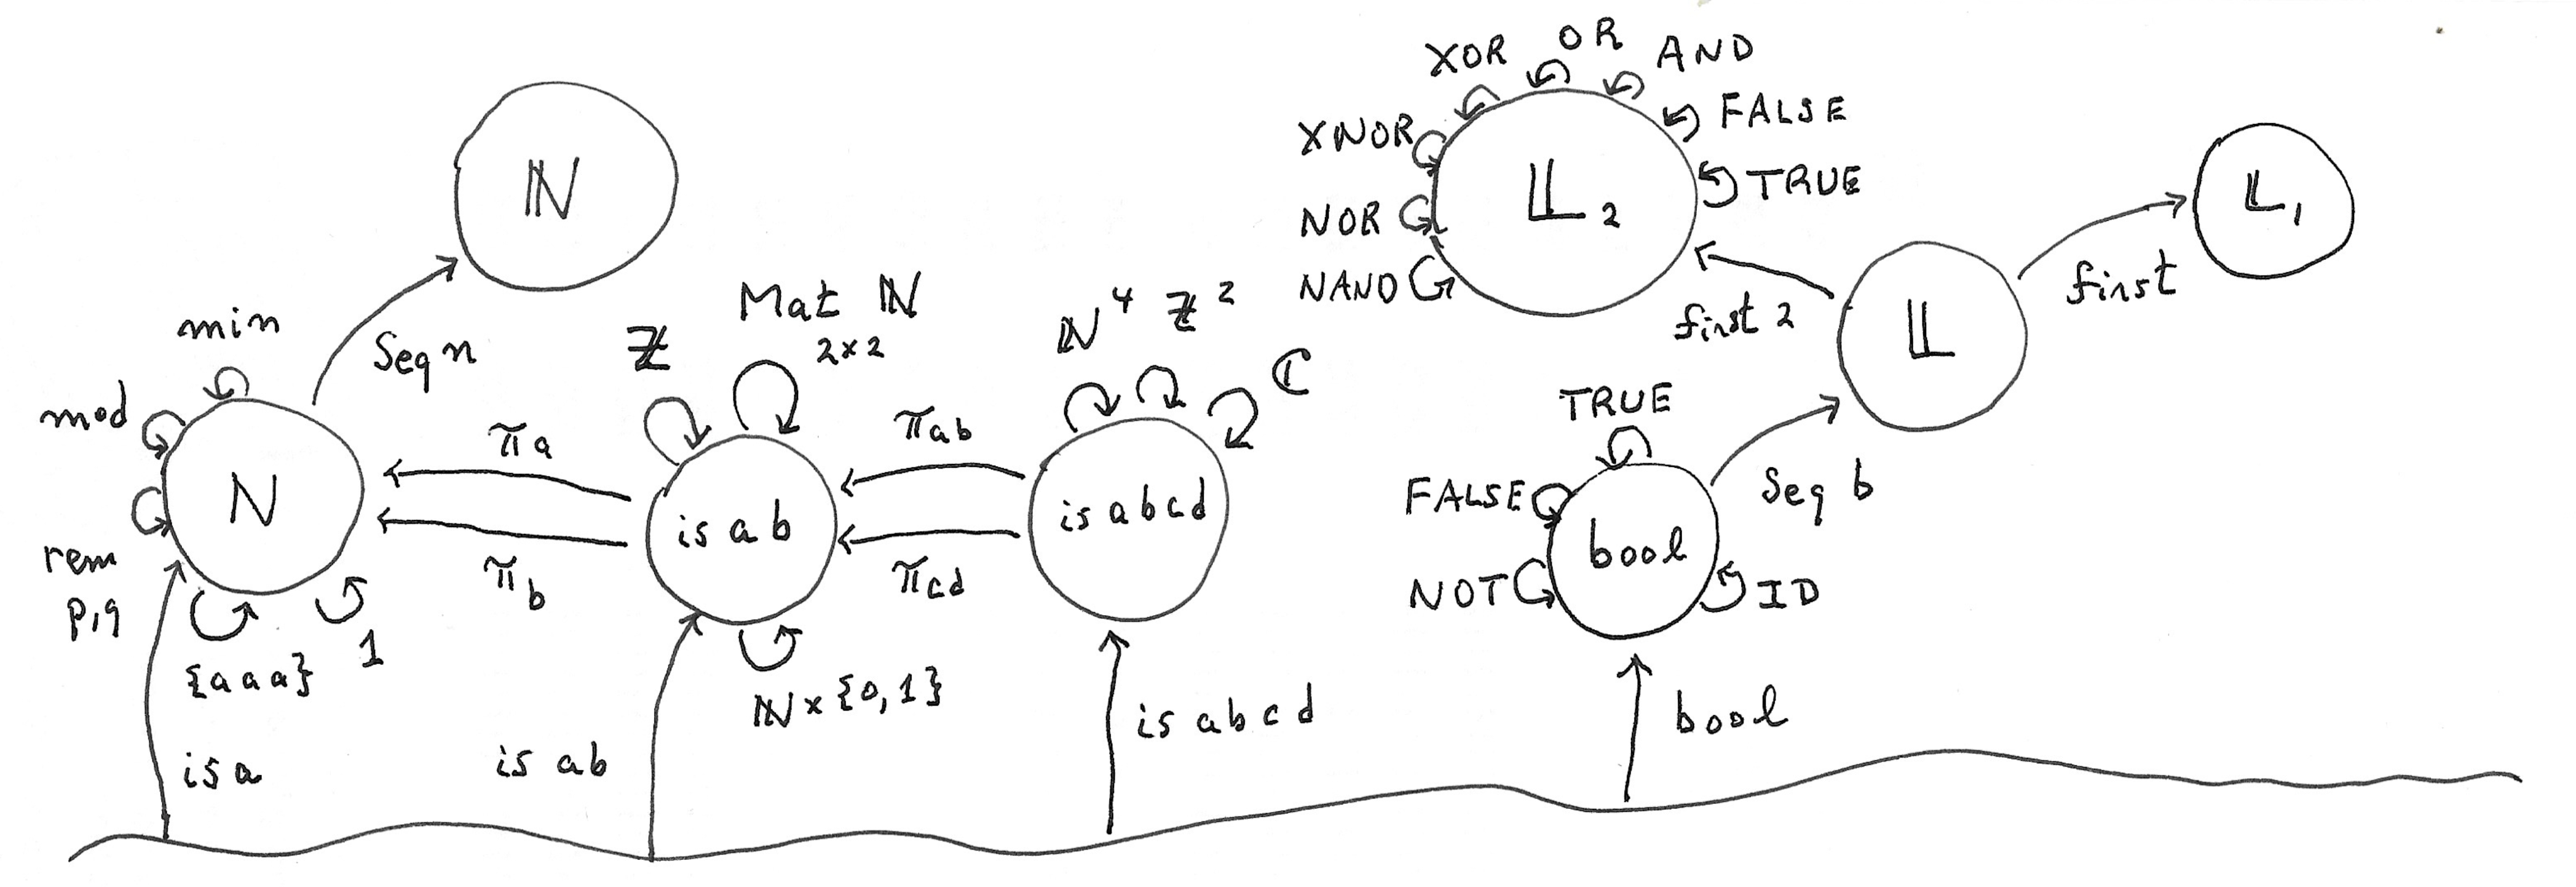
\includegraphics[width=0.8\textwidth]{garden.png}
\caption{{\it Some of the spaces and morphisms discussed in the text and ``grown organically'' from the space of all pure data. 
The main starting points are natural number spaces (central homomorphism spaces) and bool (central algebraic spaces).}}
\end{figure}

\section{Glossary}

\begin{enumerate}
\item {Basics
\begin{enumerate}
\item{$\delta_{\rm const}$ : (const A : B) $\mapsto$ A}
\item{$\delta_{\rm put}$ : (put A : B) $\mapsto$ (A:B)} 
\item{$\delta_{\rm get}$ : (get : (:B)) $\mapsto$ B....FIXME}
\item{$\delta_{\rm atoms}$ : (atoms : b B) $\mapsto$ (:)\ (atoms : B)}
\item{$\delta_{\rm bin}$ : (bin A:B) $\mapsto$ (bin A:B), atom} 
\end{enumerate}
}
\item {Control
\begin{enumerate}
\item{$\delta_{\rm if}$: (if ():B) $\mapsto$ B }
\item{$\delta_{\rm if}$: (if a A:B) $\mapsto$ () }
\item{$\delta_{\rm while}$: (while A:B) $\mapsto$ B if (A:B)=B }
\item{$\delta_{\rm while}$: (while A:B) $\mapsto$ (while A: A : B) }
\end{enumerate}
}
\item{Semiring
\begin{enumerate}
\item{prod}
\item{sum}
\end{enumerate}
}
\item{Definition}
\item{Combinatorics} 
\begin{enumerate}
\item{map}
\item{various aps}
\end{enumerate}
\item{Sequence 
\begin{enumerate}
\item{(nat:n)->n (nat:n+1), example of infinite data.  MOVE UP TO TOP?}
\item{$\delta_{\rm first}$ : (first : b B) $\mapsto$ b}
\item{$\delta_{\rm first}$ : (first : ()) $\mapsto$ ()} 
\item{$\delta_{\rm last}$ : (last : B b) $\mapsto$ b} 
\item{$\delta_{\rm last}$ : (last : ()) $\mapsto$ ()} 
\item{has}
\item{hasnt}
\item{is}
\item{isnt} 
\item{once} 
\item{$\delta_{\rm rev}$ : (rev : B b) $\mapsto$ b (rev:B)} 
\item{$\delta_{\rm rev}$ : (rev : () ) $\mapsto$ ()}
\item{rem} 
\item{sort} 
\end{enumerate} 
}
\end{enumerate}

%%%%%%%%%%%%%%%%%%%%%%%%%%%%%%%%%%%%%%%%%%%%%%%%%%%%%%%%%%%%%%%%%%%%%%%%
%%% 
\begin{thebibliography}{10}
\bibitem{PDF} {\it Pure Data Foundation of Mathematics and Computing}, Saul Youssef, 2023.
\bibitem{Berry} Nicholas Griffin (2003-06-23). {\it The Cambridge Companion to Bertrand Russell}. Cambridge University Press. p. 63. ISBN 978-0-521-63634-6.
\bibitem{Mazur} Barry Mazur, {\it When is one thing equal to some other thing?}, Harvard University, 2007,  {\rm https://people.math.harvard.edu/}$\sim${\rm mazur/preprints/when\_is\_one.pdf}. 
\end{thebibliography}
%%%%%%%%%%%%%%%%%%%%%%%%%%%%%%%%%%%%%%%%%%%%%%%%%%%%%%%%%%%%%%%%%%%%%%%%
\end{document}
